\section{Introduction}

The difference between computer vision and image processing is the fact that computer vision is the process of extracting information from images, while image processing aims at improving the quality of images.
Quite often image processing helps computer vision.
The informations we want to extract from the images could be counting, object orientation, object classification, measurements...
Computer vision is challenging since we lose depth from the images (3D information becomes 2D), scale and illumination varies, and there's object occlusion (object hiding other objects).

Computer vision started with hand-crafted decision rules that only required few images as example, and evolved to machine learning where the algorithm learns a decision rule, but the training requires hundreds to thousands of images.
The big paradigm shift happened with deep learning (e2e learning) which learned both the image representation and the decision rules, but required thousands to millions of words.
Deep learning has been enabled by better networks, better hardware and more data.


\section{Fundamentals of Image Processing and Computer Vision}
% lecture 2

\subsection{Images}

An imaging device gathers the light reflected by 3D objects to create a 2D representation of the scene.

\subsubsection{Pinhole camera model}
The "pinhole camera" is the simplest camera model we can define.
Light goes through the very small pinhole (to not have saturation) and hits the image plane.
Geometrically, the image is achieved by drawing straight rays from scene points through the hold up to the image plane.

This simple geometrical model turns out to be a good approximation of the geometry of image formation.
However, useful images can hardly be captured by means of a pinhole camera.

The \textbf{geometric model of image formation} in a pinhole camera is known as \textbf{perspective projection}.

\begin{figure}[htbp]
  \centering
  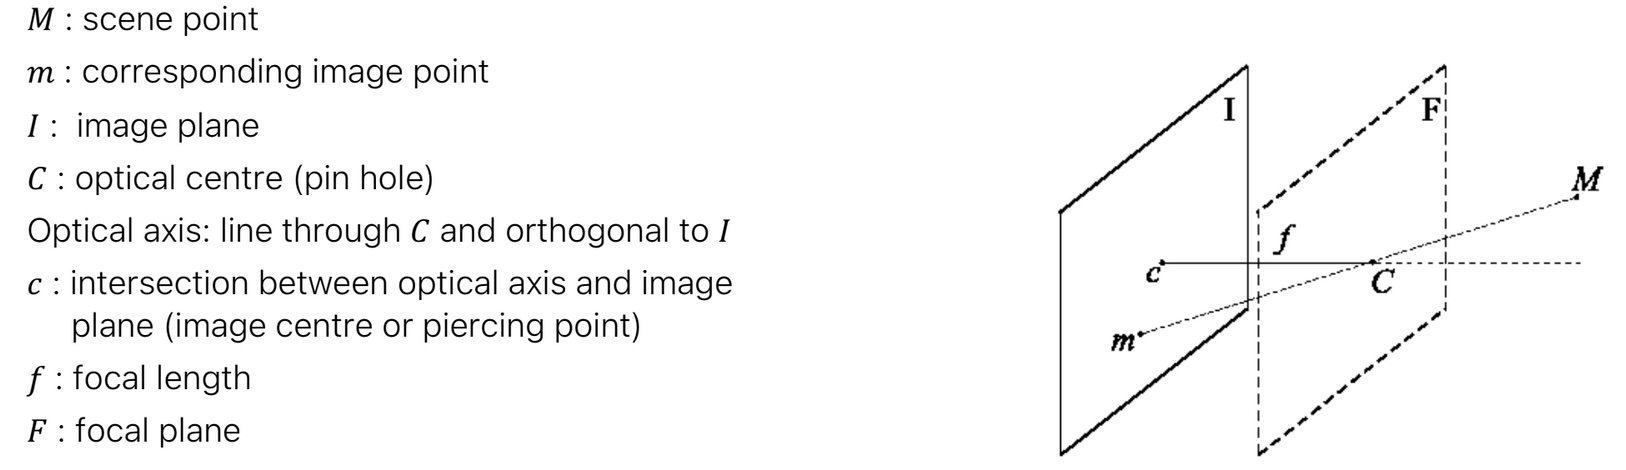
\includegraphics[width=0.9\linewidth]{./img/perspective_projection.jpg}
  \caption{perspective projection}
\end{figure}

Which, by writing the points as vectors and the plane's coordinates, becomes the geometric model in the image \ref{fig:perspective_projection_axis}

\begin{figure}[htbp]
  \centering
  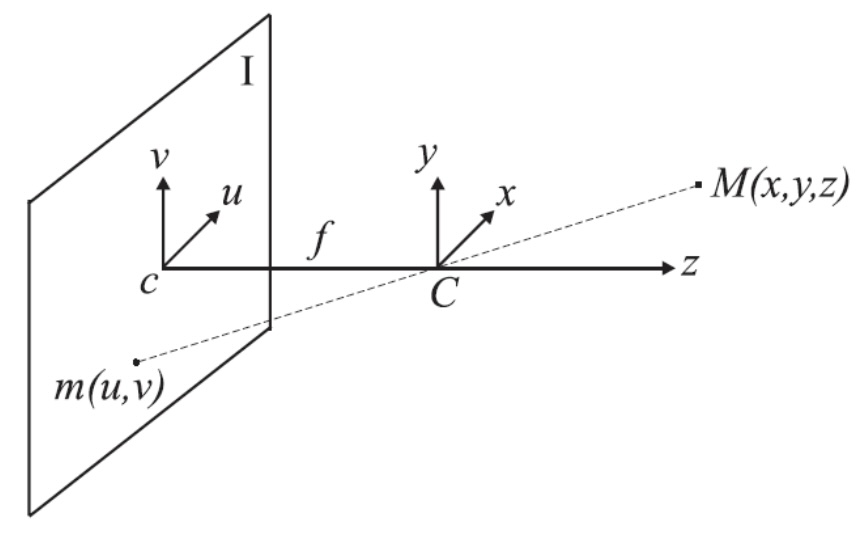
\includegraphics[width=0.45\linewidth]{./img/perspective_projection_axis.jpg}
  \caption{geometric model of image formation}
  \label{fig:perspective_projection_axis}
\end{figure}

Given the reference frame in the image \ref{fig:perspective_projection_axis} 
\begin{itemize}
  \item $u$ is the horizontal axis in the image plane.
  \item $v$ is the vertical axis in the image plane.
   \item $x$ and $y$ are the respective axis in the 3D reference system. It's called the \textbf{camera reference system} because it is "attached" to the camera.
\end{itemize}

\textbf{For the perspective model these axis must be parallel}

The equations to map scene points into their corresponding image points are defined as:

$$\frac{u}{x} = -\frac{f}{z} \rightarrow u = -x\frac{f}{z} \quad\quad\quad \frac{v}{y} = - \frac{f}{z} \rightarrow v = -y\frac{f}{z}$$

The minus sign means the axis gets inverted (as we can see in the visualization, and it's what happens in the brain).
We can get rid of the sign, since the image plane can be though of as lying in front rather than behind the optical centre.

Image coordinates are a scaled version of scene coordinates (function of depth).
When $z$ increases, since it's at the denominator in both the equations, the terms gets smaller (object gets smaller in the image).
When $f$ increases, since it's at the numerator in both the equations the term gets bigger (object gets bigger in the image)

As we previously said, the image formation process deals with mapping a 3D space onto a 2D space, and so to the loss of depth information.
A given scene point is mapped into an image point, but an image point is mapped onto a 3D line.
For an image point we can only state that its corresponding scene point lays on a line, but cannot disambiguate a specific 3D point along the line.

\subsubsection{Stereo images}

We use multiple images to create stereo vision.
Given correspondences, 3D information can be recovered easily by triangulation.
We can use two cameras, or two cameras and an infrared sensor to project guides to align the images.

For standard stereo geometry there are some assumptions we have to make:
\begin{itemize}
  \item The cameras have parallel $(x,y,z)$ axes.
  \item The image planes of both cameras are coplanar and aligned.
  \item Both cameras have identical focal lengths.
\end{itemize}
\vspace{1em}
Based on this, the transformation between the two reference frames is just a translation, usually horizontal.
For stereo vision is also really important to \textbf{sense two images at the same moment}.

The cameras are displaced at a given quantity $b$ called baseline.
The \textbf{disparity} is the difference between the horizontal coordinates in the left and right images.

\begin{figure}[htbp]
  \centering
  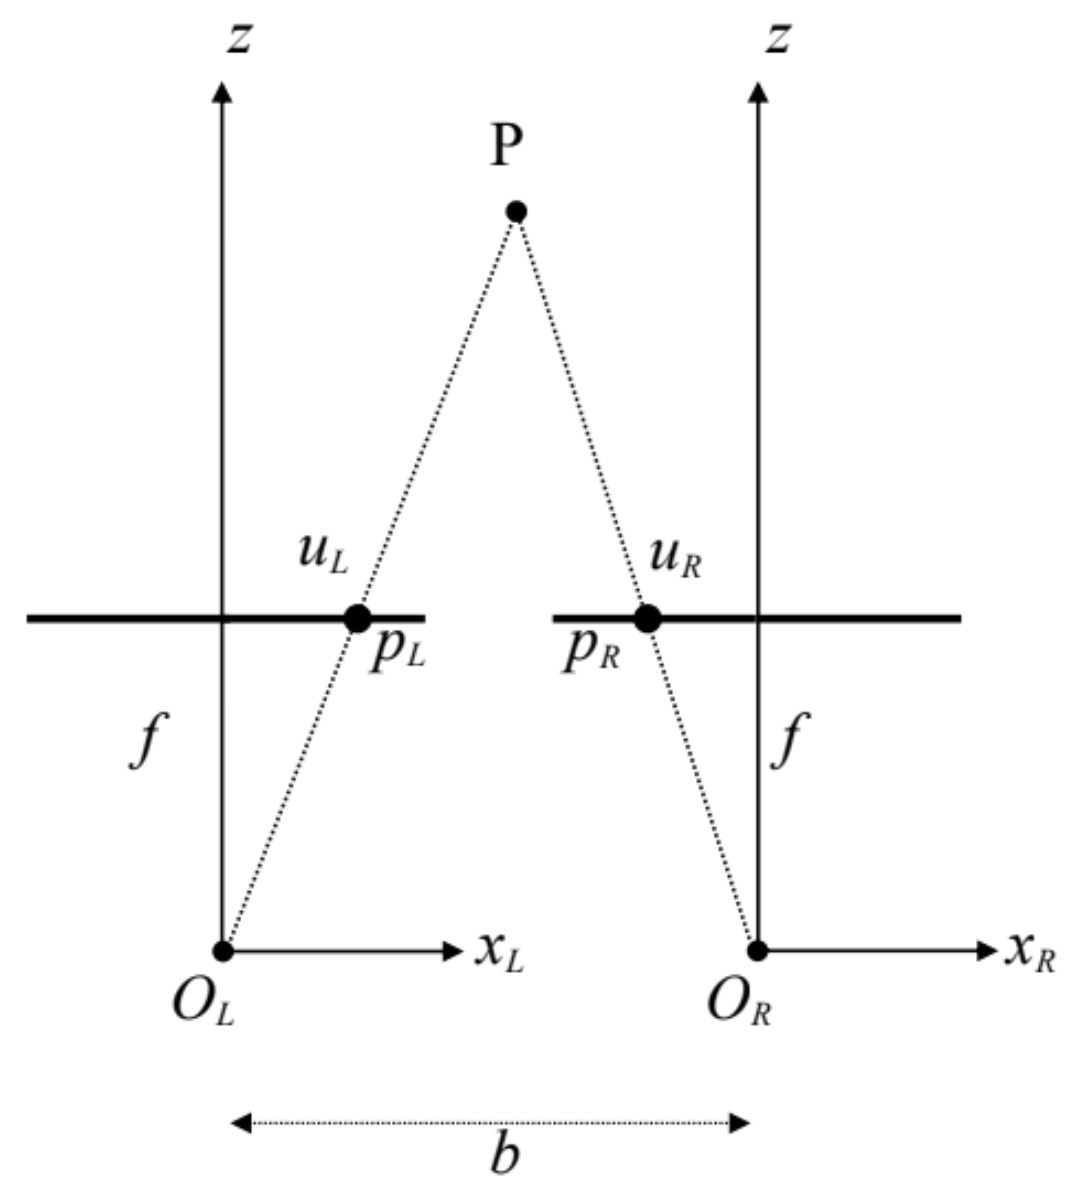
\includegraphics[width=0.45\linewidth]{./img/standard_stereo_geometry.jpg}
  \caption{standard stereo geometry}
  \label{fig:standard_stereo_geometry}
\end{figure}

% The fundamental relationship in stereo vision is $z = b \cdot \frac{f}{d}$.
% It's used to calculate the depth of a point in a scene from a pair of stereo images.

In standard stereo geometry since we are given just two 2D images there is no info about the correspondence between two points in the two images.
We can recall that the camera have parallel axes, and so we know that we can search for the correspondence along the horizontal lines.
This task is called stereo matching.

\subsubsection{Stereo correspondence}
In stereo correspondence, given a point in one image, we have to find it in the other image which is the projection of the same 3D point.
Such image points are called corresponding points.
\textbf{Points farther away have a smaller disparity, while close points have a larger disparity}.

\begin{figure}[htbp]
  \centering
  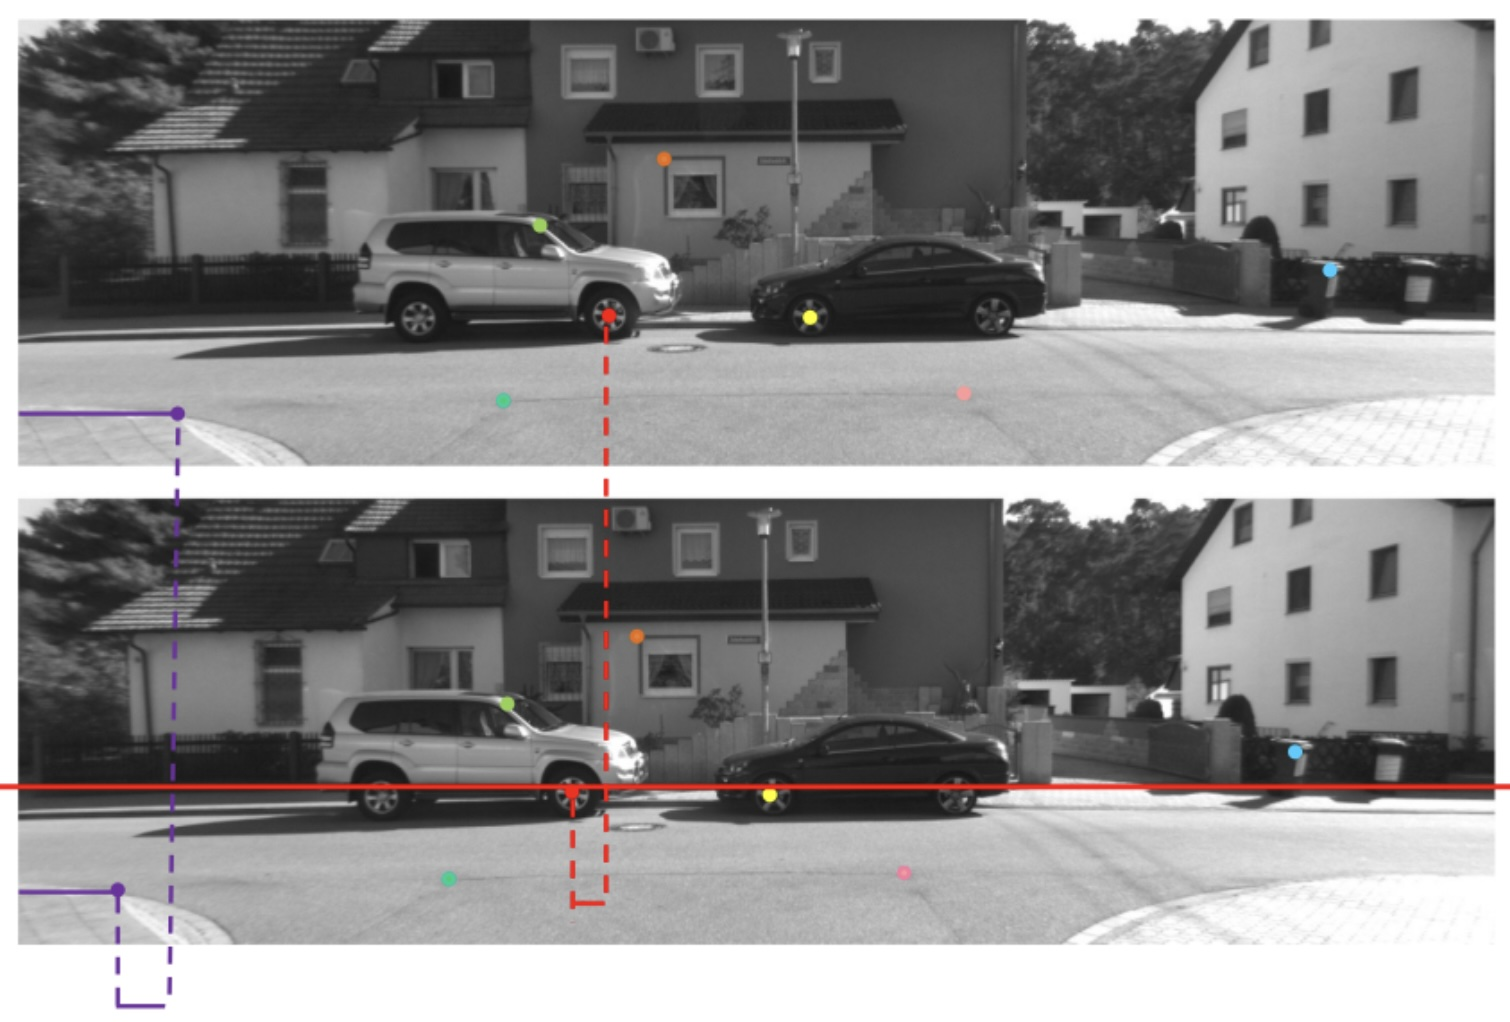
\includegraphics[width=0.65\linewidth]{./img/stereo_correspondence.jpg}
  \caption{Corresponding points look similar in the two images}
  \label{fig:stereo_correspondence}
\end{figure}

The image of a 3D line segment of length $L$ lying in a plane parallel to the image plane at distance $z$ from the optical centre will exhibit a length given by:
$$l = L \frac{f}{z}$$
This relationship is more complicated for an arbitrarily oriented 3D segment, as its position and orientation need to be accounted for as well.
For a \textbf{given position and orientation, length always shrinks alongside distance}.

Perspective projection maps 3D lines into image lines.
\textbf{Parallelism between 3D lines is not preserved} (except for lines parallel to the image plane).
This is the reason why if we look at a really long road into the distance we have the perception that the road becomes thinner, and the lines of the road intersect in the distance.
The images of parallel 3D lines intersect at a point, called \textbf{vanishing point}, which isn't necessarily within the image.

If the lines are parallel to the image plane they meet at infinity.

\subsubsection{Epipolar geometry}

What if the two cameras are no longer aligned? Do we need to search through the whole image?
We can project the line related to point $P_L$ in the right plane and search across that line.
The issue is that this projection can be computed only if the transformation between the two cameras is known (the relative mapping between the two cameras).

\begin{figure}[htbp]
  \centering
  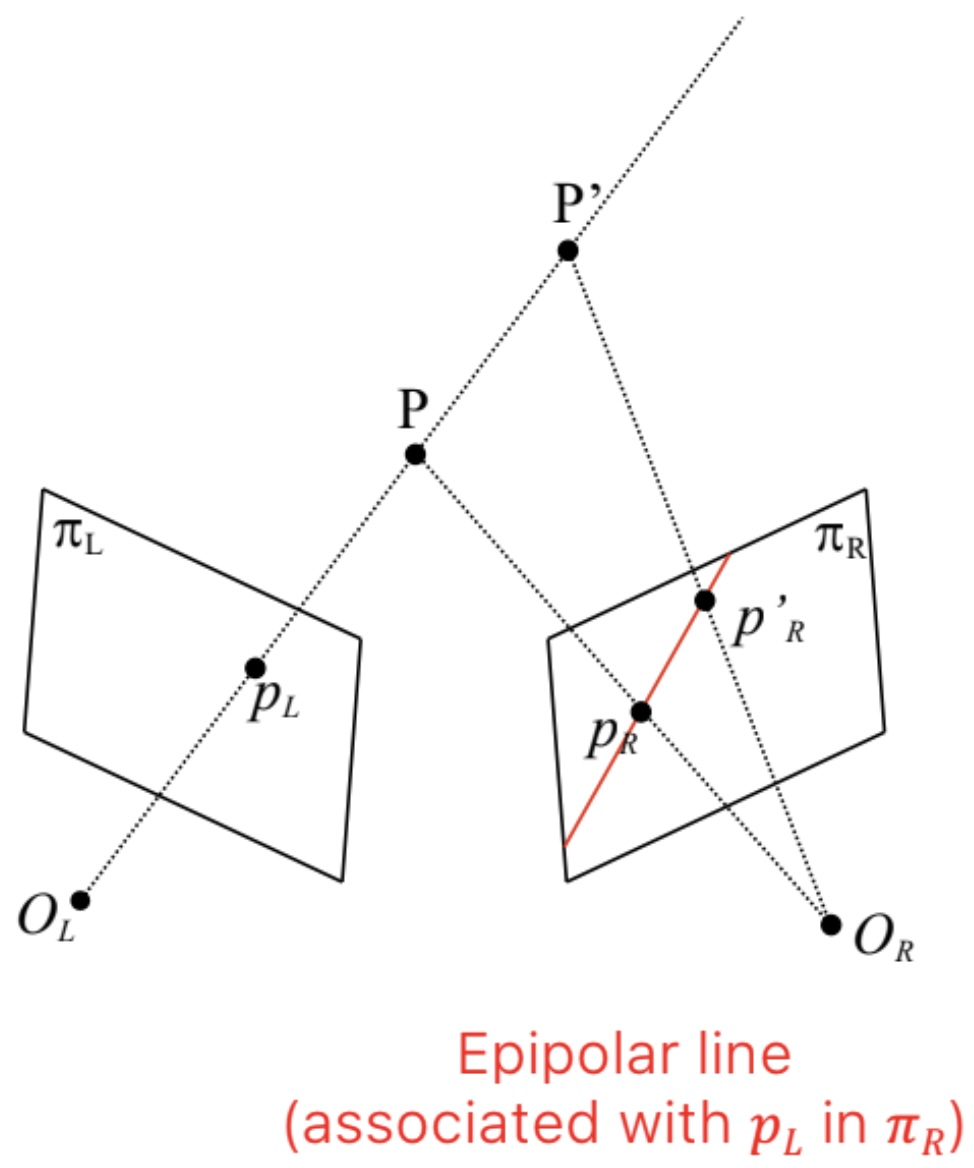
\includegraphics[width=0.45\linewidth]{./img/epipolar_line.jpg}
  \caption{Epipolar line}
  \label{fig:epipolar_line}
\end{figure}

It is almost impossible to build a stereo rig which is perfectly aligned horizontally.
Searching through oblique epipolar lines is awkward, and computationally is less efficient.
What people do in practice is to convert epipolar geometry to standard geometry with rectification/warping.
We warp the images as if they were acquired through a standard geometry, then we can compute and apply to both images a transformation known as rectification.

\subsubsection{Depth of Field (DOF)}

A scene point is on focus when all its light rays, gathered by the camera, hit the image plane at the same point.
In a pinhole device this happens to all scene points because of the very small size of the hole, so that the camera features an infinite Depth of Field (DOF).

The drawback is that such a small aperture allows gathering a very limited amount of light.
The image is really sharp, but has a really low light.
If a point is projected onto a circle instead of a point (bigger pinhole) the image is not sharp (not on focus).
If we cannot gather enough light through the aperture we have to integrate through time, by using a longer exposure time.

\subsubsection{Lenses}

Lenses concentrate light, so we use them to gather more light from a scene point and focus it on a single image point.
This enables much smaller exposure times.
This way Depth Of Field is no longer infinite, and only a limited range of points can be simultaneously on focus in a given image.

We will consider the approximate model known as thin lens equation, which is useful to graphically determine the position of a focused image point:
\begin{itemize}
  \item Rays parallel to the optical axis are deflected to pass through $F$.
  \item Rays through $C$ are undeflected.
\end{itemize}

\textbf{If the image is on focus}, the image formation process obeys to the perspective projection model:
\begin{itemize}
  \item The center of the lens is the optical center.
  \item The distance $v$ acts as the effective focal length of the projection.
\end{itemize}

\begin{figure}[htbp]
  \centering
  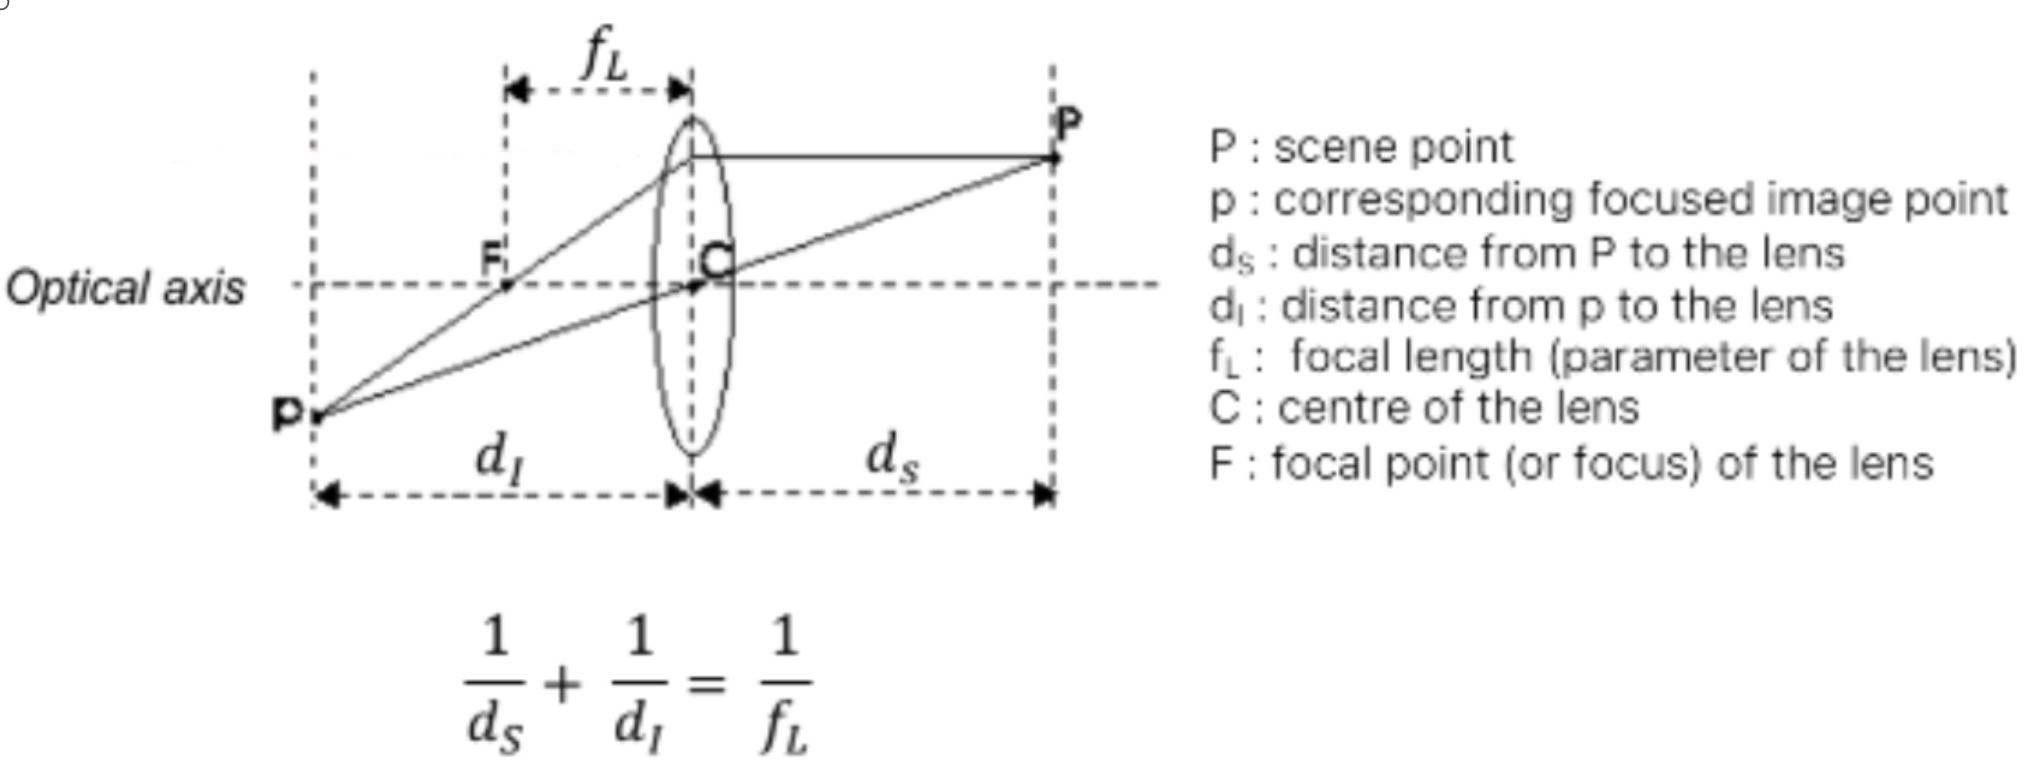
\includegraphics[width=0.7\linewidth]{./img/lens.jpg}
  \caption{Scheme of a lens}
  \label{fig:lens}
\end{figure}

Choosing the distance of the image plane determines the distance at which scene points appear on focus in the image.
Scene points in front and behind the focusing plane will result out-of-focus, thereby appearing in the image as \textbf{blur circles}, rather than points.

The advantage of lenses is to have a small exposure time for capturing moving objects but we pay in terms of Depth Of Field.

\begin{figure}[htbp]
  \centering
  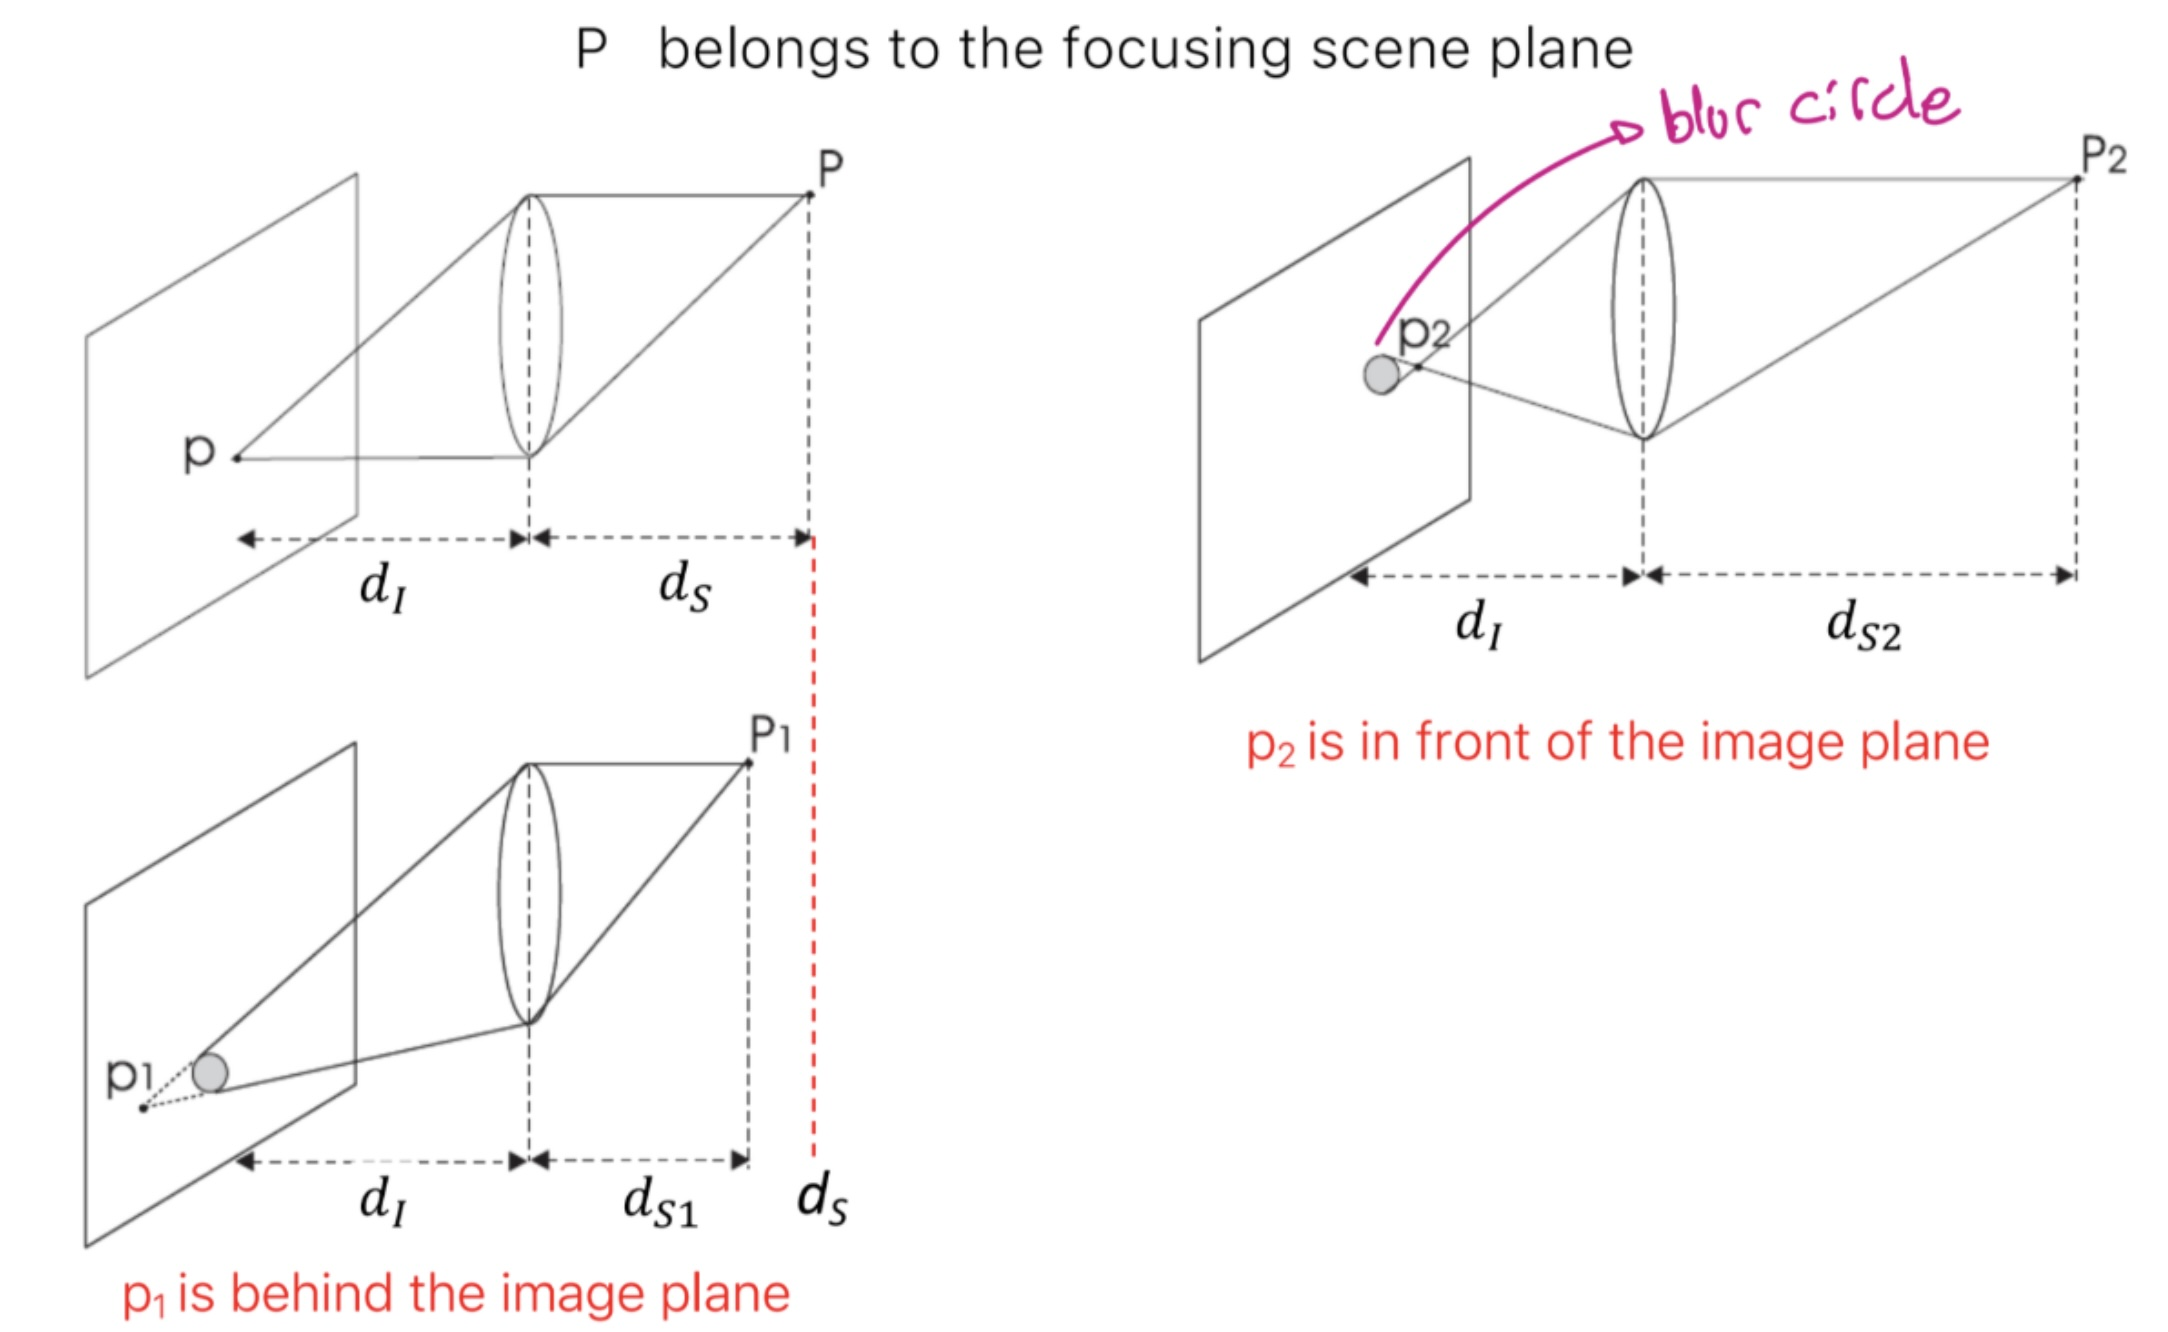
\includegraphics[width=0.8\linewidth]{./img/lens_focus.jpg}
  \caption{Lens focusing at various distances}
  \label{fig:lens_focus}
\end{figure}

As we can see in \ref{fig:tradeoffs} having a small aperture (pinhole camera model) results in everything being on focus, but we need lots of light, or the image will be dark, since few light can enter in the sensor.
We could also increase our exposure time to let more light in, but in that case we need the objects in our image to be still.
Having a bigger aperture results in more light coming in in a small time fraction, but the lens distortion causes the light to be focused only at certain distances, and creates blur cirlces in other zones, so we get a lower depth of field, as we can see in \ref{fig:lens_focus}.

\begin{figure}[htbp]
  \centering
  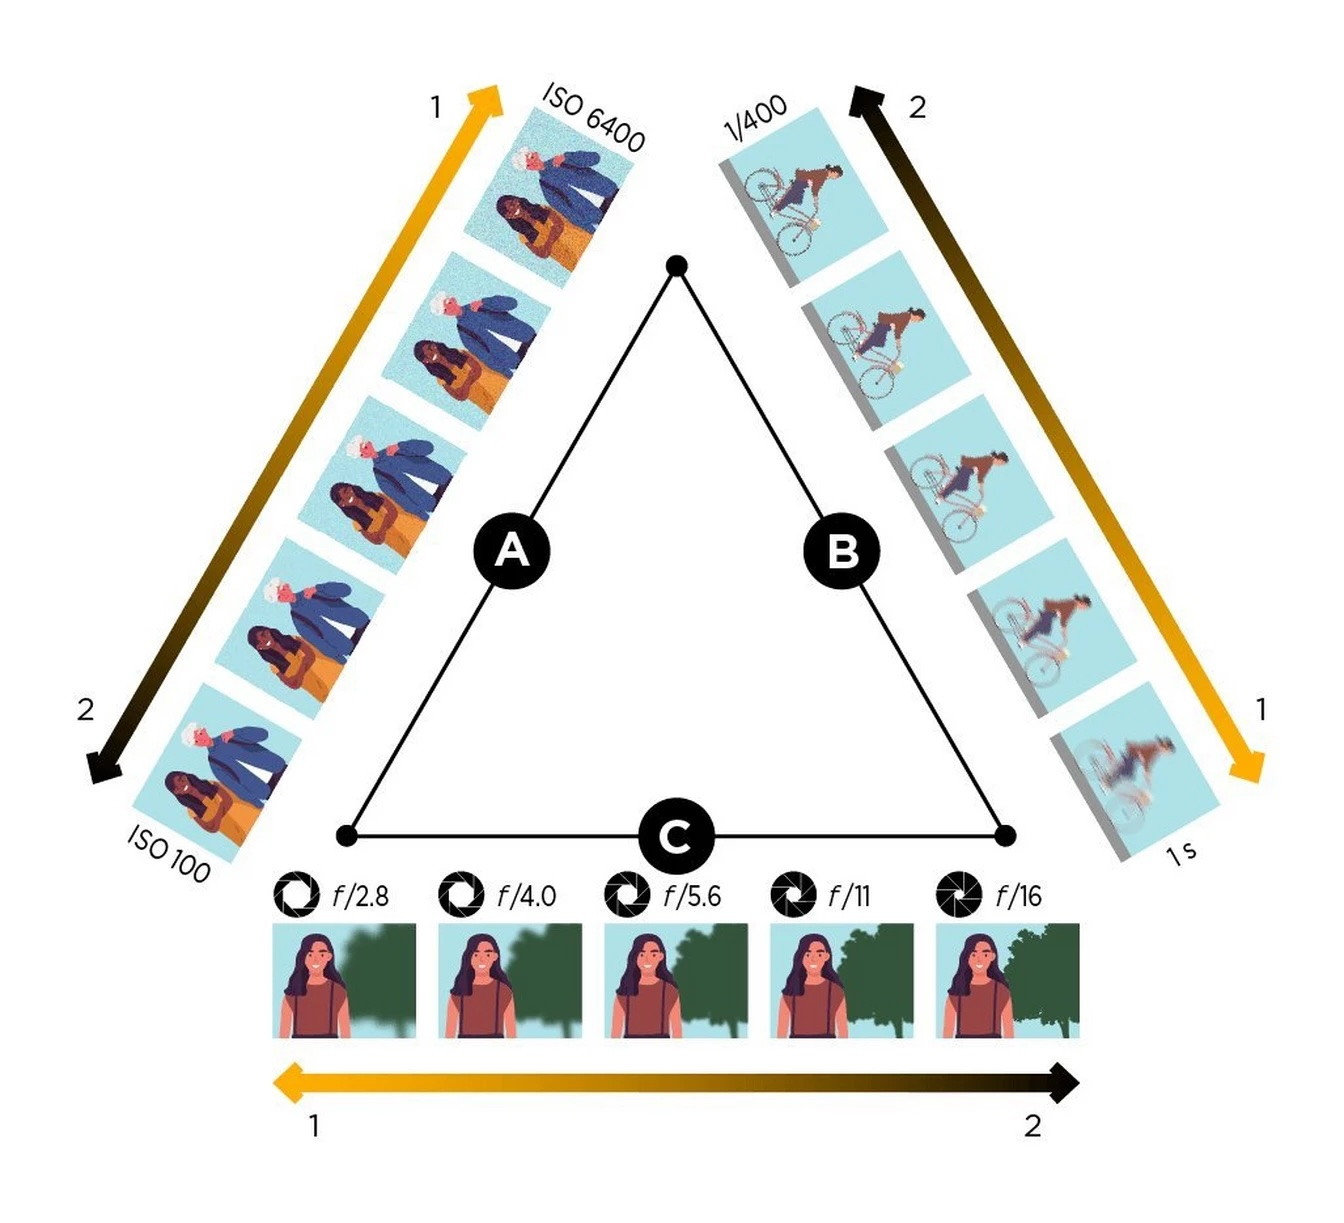
\includegraphics[width=0.8\linewidth]{./img/tradeoffs.jpg}
  \label{fig:tradeoffs}
\end{figure}

\subsubsection{Diaphragm}

In theory, when imaging a scene through a thin lens, only the points at a certain distance can be on focus, all the others appear blurred into circles.
However, as long as the circles are smaller than the size of the photosensing elements (a single pixel), the image will still look on-focus.

\begin{figure}[htbp]
  \centering
  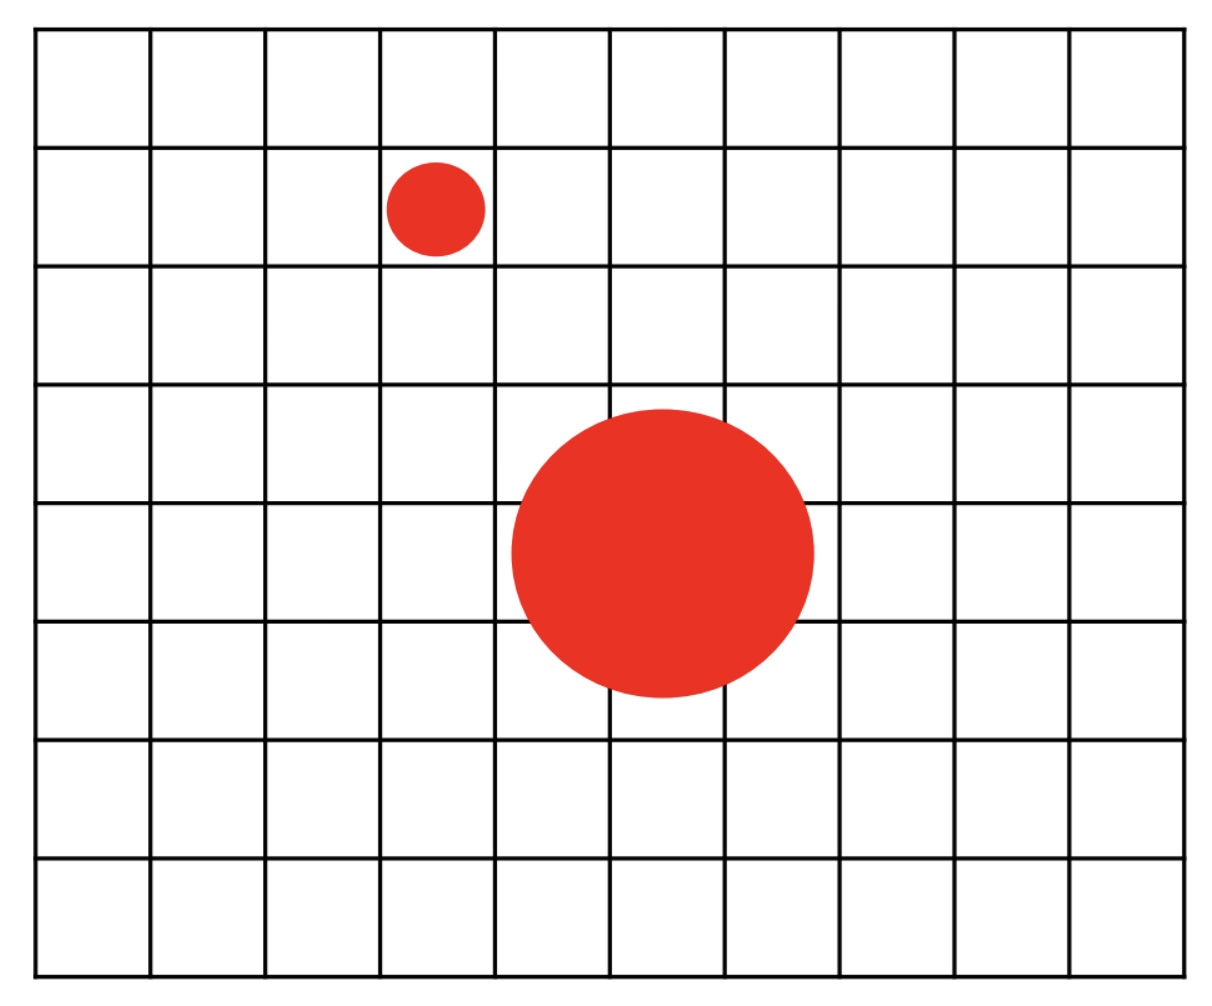
\includegraphics[width=0.55\linewidth]{./img/diaphragm.jpg}
  \caption{Blurring at pixel level}
  \label{fig:diaphragm}
\end{figure}

The range of distances across which the image appears on focus, due to blur circles being small enough, determines the (Depth Of Field) of the imaging apparatus.
Cameras often deploy an adjustable diaphragm (iris) to control the amount of light gathered through the effective aperture of the lens.
\begin{itemize}
  \item Reduce aperture $\rightarrow$ less light $\rightarrow$ smaller blur circle
  \item More aperture $\rightarrow$ more light $\rightarrow$ larger blur circle.
  \item Close the diaphragm $\rightarrow$ increase depth of field $\rightarrow$ not enough light $\rightarrow$ increase exposure time $\rightarrow$ moving object $\rightarrow$ motion blur.
\end{itemize}

\subsubsection{Focusing mechanism (manually changing depth of field)}
To focus on objects at diverse distances we need a mechanism that allows the lens (or the lens subsystem) to translate along the optical axis with respect to the fixed position of the image plane.

\begin{figure}[htbp]
  \centering
  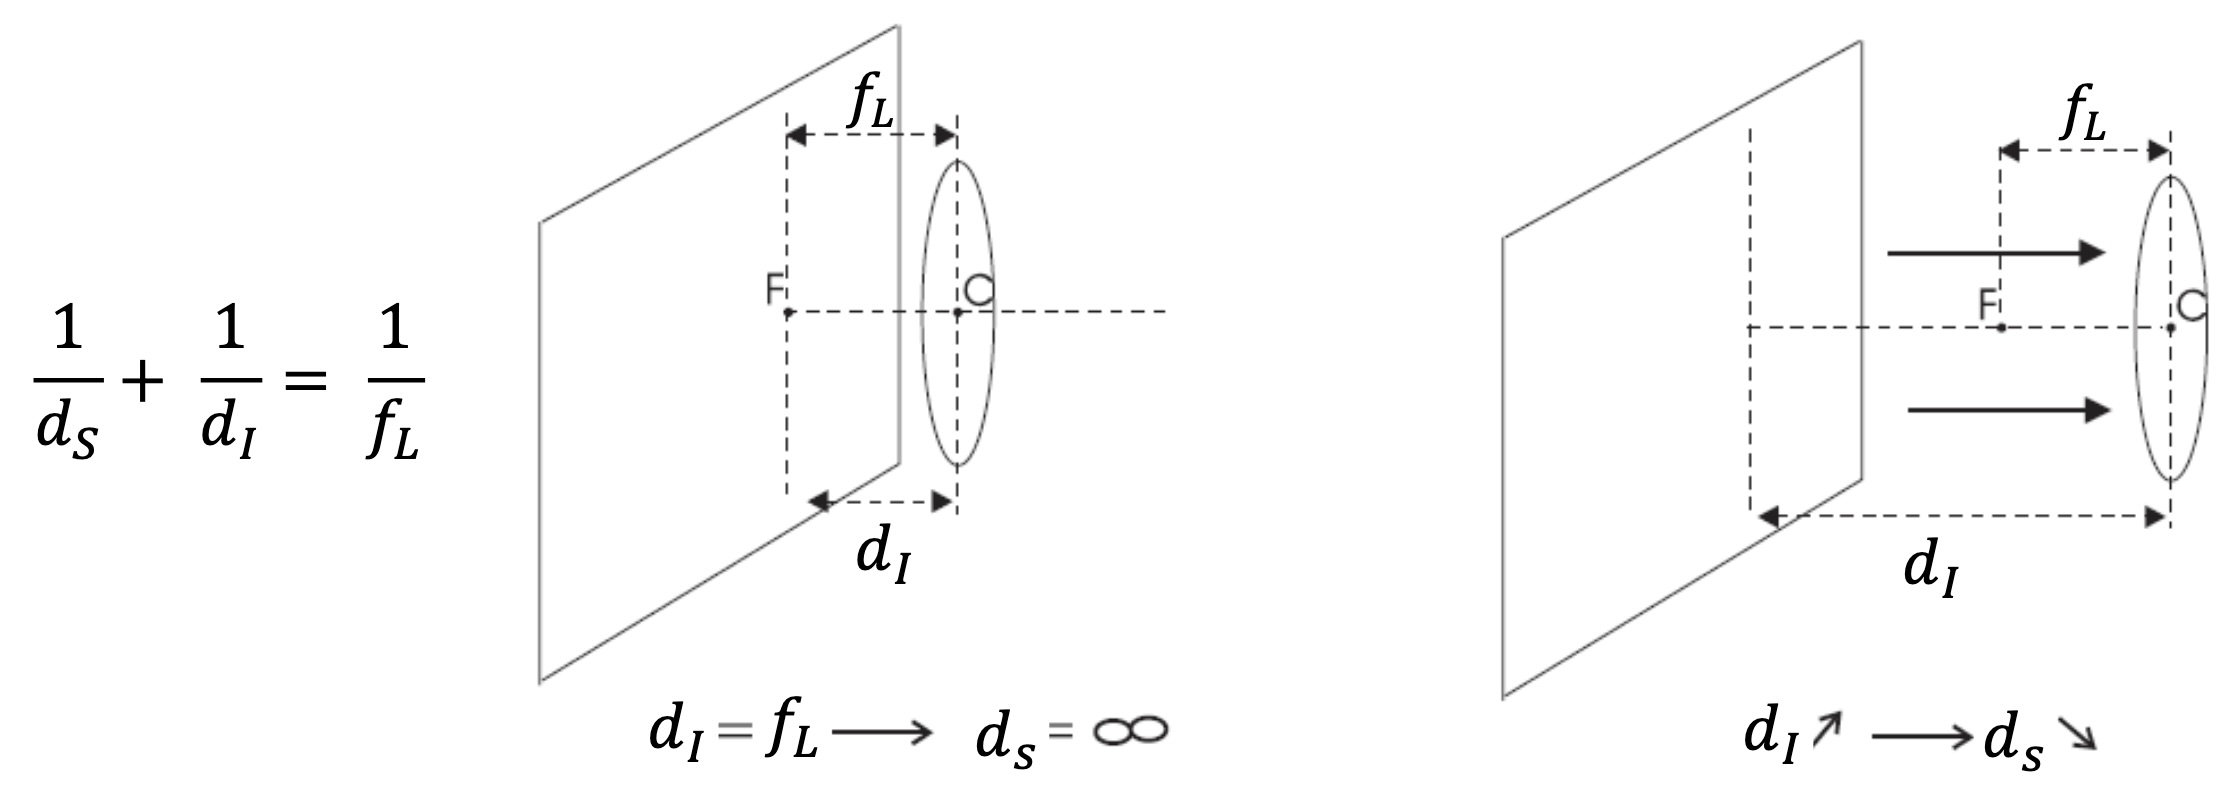
\includegraphics[width=0.7\linewidth]{./img/focusing_mechanism.jpg}
  \caption{Focusing mechanism}
  \label{fig:focusing_mechanism}
\end{figure}

At one end position ($d_I = f_L$) the camera is focused at infinity (objects at inifity are on sharp focus).
The focusing mechanism allows the lens to be translated farther away from the image plane up to a certain maximum value, which determines the minimum focusing distance.

\subsubsection{Image digitization}

How do we convert a continuous image to a discrete one which can be represented on a computer? 
The process can be divided in two steps: sampling and quanitzation.

\begin{figure}[htbp]
  \centering
  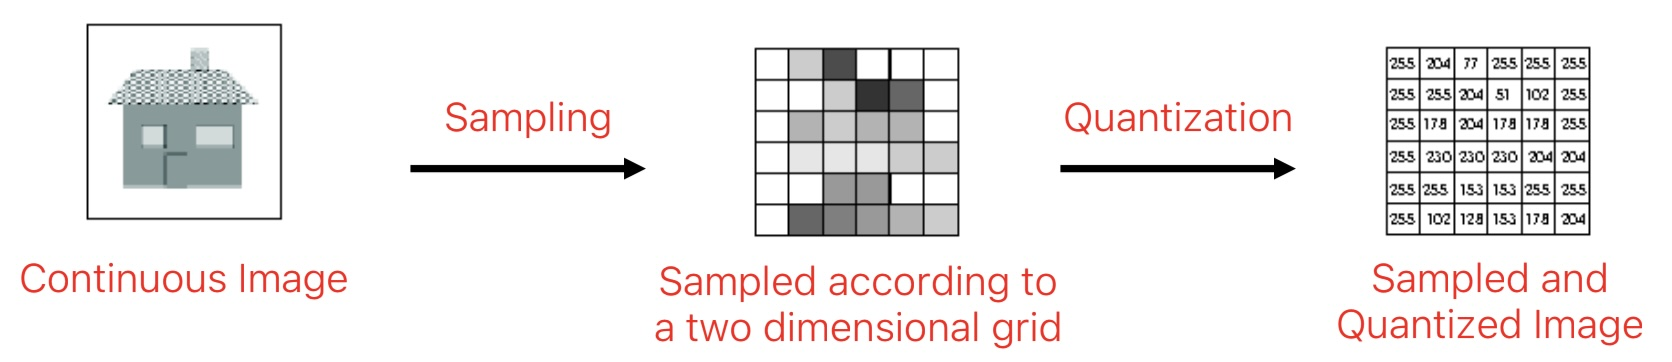
\includegraphics[width=0.55\linewidth]{./img/image_digitization.jpg}
  \caption{The two steps of the image digitization process}
  \label{fig:image_digitization}
\end{figure}

\begin{itemize}
  \item \textbf{Sampling}: the planar continuous image is sampled along both the horizontal and vertical directions to pick up a matrix of $N\times M$ samples (pixels).
  \item \textbf{Quantization}: the continuous range of values associated with pixels is quantized into $l=2^m$ discrete levels known as gray-levels.
  $m$ is the number of bits used to represent a pixel, with the memory occupancy (in bits) of a gray-scale image given by $B = N \times M \times m$. Coloured digital images are typically represented within computers using 3 bytes per pixels. Both more pixels and more bits per pixel result in a higher quality image.
\end{itemize}

The more bits we spend for its representation, the higher the quality of the digital image (it becomes a closer approximation to the ideal continuous image).
This applies both to sampling and quantization.

\subsubsection{Camera sensors}

The sensor is a matrix of photodetectors.
During exposure time, each detector converts the incident light into a proportional electic charge.
The companion circuitry reads-out the charge to generate the output signal, which can be either digital or analog.
For digital cameras the sensor includes the necessary ADC circuitry.

Today, the two main sensor technologies are:
\begin{itemize}
  \item \textbf{Charge Coupled Devices (CCD)}, where the sensor and circuit are separated.
  \item \textbf{ Complementary Metal Oxide Semiconductor (CMOS)}, where everything is on the same circuit.
\end{itemize}

CCD/CMOS sensors can't sense colors, so we place an array of optical filters in front of the photodetectors, to render each pixel sensitive to a specific range of wavelengths.

\subsubsection{SNR}

The intensity measured at a pixel under perfectly static conditions varies due to the presence of random noise.
The main noise sources are:
\begin{itemize}
  \item \textbf{Photon Shot Noise}: the number of photons collected during exposure time is not constant.
  \item \textbf{Electronic Circuitry Noise}: generated by the electronics.
  \item \textbf{Quantization Noise}: related to the ADC conversion.
  \item \textbf{Thermal Noise (Dark Current Noise)}: random charge observed due to thermal excitement.
\end{itemize}

SNR can be expressed both in decibels and bits.

\subsubsection{Dynamic Range (DR)}
If the sensed amount of light is too small, the "true" signal cannot be distinguished from noise.
Given $E_{\text{min}}$: the minimum detectable irradiation, and $E_{\text{max}}$, the saturation irradiation.
The Dynamic Range (DR) of a sensor is defined as $DR = \frac{E_{\text{max}}}{E_{\text{min}}}$, and like the SNR, it is often specified in decibels or bits.

Like SNR, the higher the DR the better it is.
A \textbf{higher DR} corresponds to the ability of the sensor to simultaneously \textbf{capture in one image both the dark and bright} structures of the scene.

% lecture 2 part 2
\subsection{Image Filtering}

\subsubsection{Noise and image filters}

In computer vision we have to deal with noise.
Noise is always different, and more noticeable in uniform regions of the image.
The simplest thing to reduce noise is to output the average of the pixel color over time, to get \textbf{almost} the ideal noiseless value.
$$O(p) = \frac{1}{T} \sum_{t=1}^{T} I_k(p) = \frac{1}{T} \sum_{t=1}^{T}(\tilde{I}(p) + n_t(p))$$

This technique works well on still images.

\begin{figure}[htbp]
  \centering
  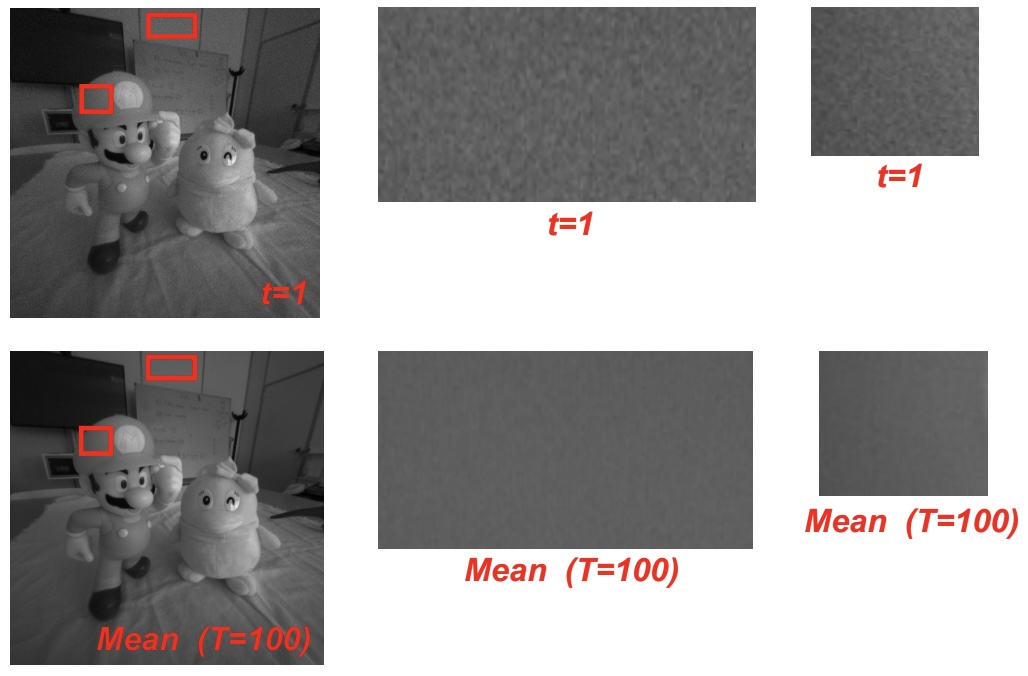
\includegraphics[width=0.7\linewidth]{./img/denoising_simple.jpg}
  \caption{Simple denoising}
  \label{fig:denoising_simple}
\end{figure}

If we are given a simple image, we may compute a mean across neighbouring pixels, like a spatial rather than temporal mean.
The size of the square of the neighbouring pixels is a tradeoff.

This is a very basic denoising filter.

Image filters are image processing operators that compute the new intensity (colour) of a pixel, $p$, based on the intensities (colours) of those belonging to a neighbourhood (support) of $p$.

\subsubsection{Convolution}

An important sub-class of filters is given by \textbf{Linear} and \textbf{Translation-Equivariant (LTE)} operators.

The \textbf{application of filters} in image processing consists in a \textbf{2D convolution} between the input image and the impulse response function of the LTE operator.

LTE operators are used as feature extractors in Convolutional Neural Networks (CNNs).

Given an input 2D signal $i(x,y)$, a 2D operator $T{i(x,y)}$ is said to be \textbf{linear} if and only if:
 
$$T\{\alpha i_1(x,y) + \beta i_2(x,y)\} = \alpha o_1(x,y) + \beta o_2(x,y)$$

with $o_1 = T{i_1}$ and $o_2 = T{i_2}$ and $\alpha, \beta$ are two constants.
This means that \textbf{scaling and adding images before applying the filter gives the same result as filtering them separately} and then scaling and adding the results.

The operator is said to be \textbf{translation-equivariant} if and only if:
$$T\{i(x-x_0, y-y_0)\} = o(x-x_0, y-y_0)$$
This means that \textbf{shifting the input shifts the output; the shape stays the same, just in a different location}.

If an operator is both linear and translation-equivariant (LTE), then its output can be written as a convolution between the input signal $i(x,y)$ and the impulse response of the system (which is the output the system gives when you input a single point)

This impulse response is written as $h(x,y) = T{\delta (x,y)}$, and the output is $o(x,y) = i(x,y) * h(x,y)$.

Mathematically, the 2D convolution is written as:
$$i(x,y) * h(x,y) = \int_{-\infty}^{\infty} \int_{-\infty}^{\infty} i(\alpha, \beta) h(x-\alpha, y-\beta) \, d\alpha  d\beta $$

\begin{figure}[htbp]
  \centering
  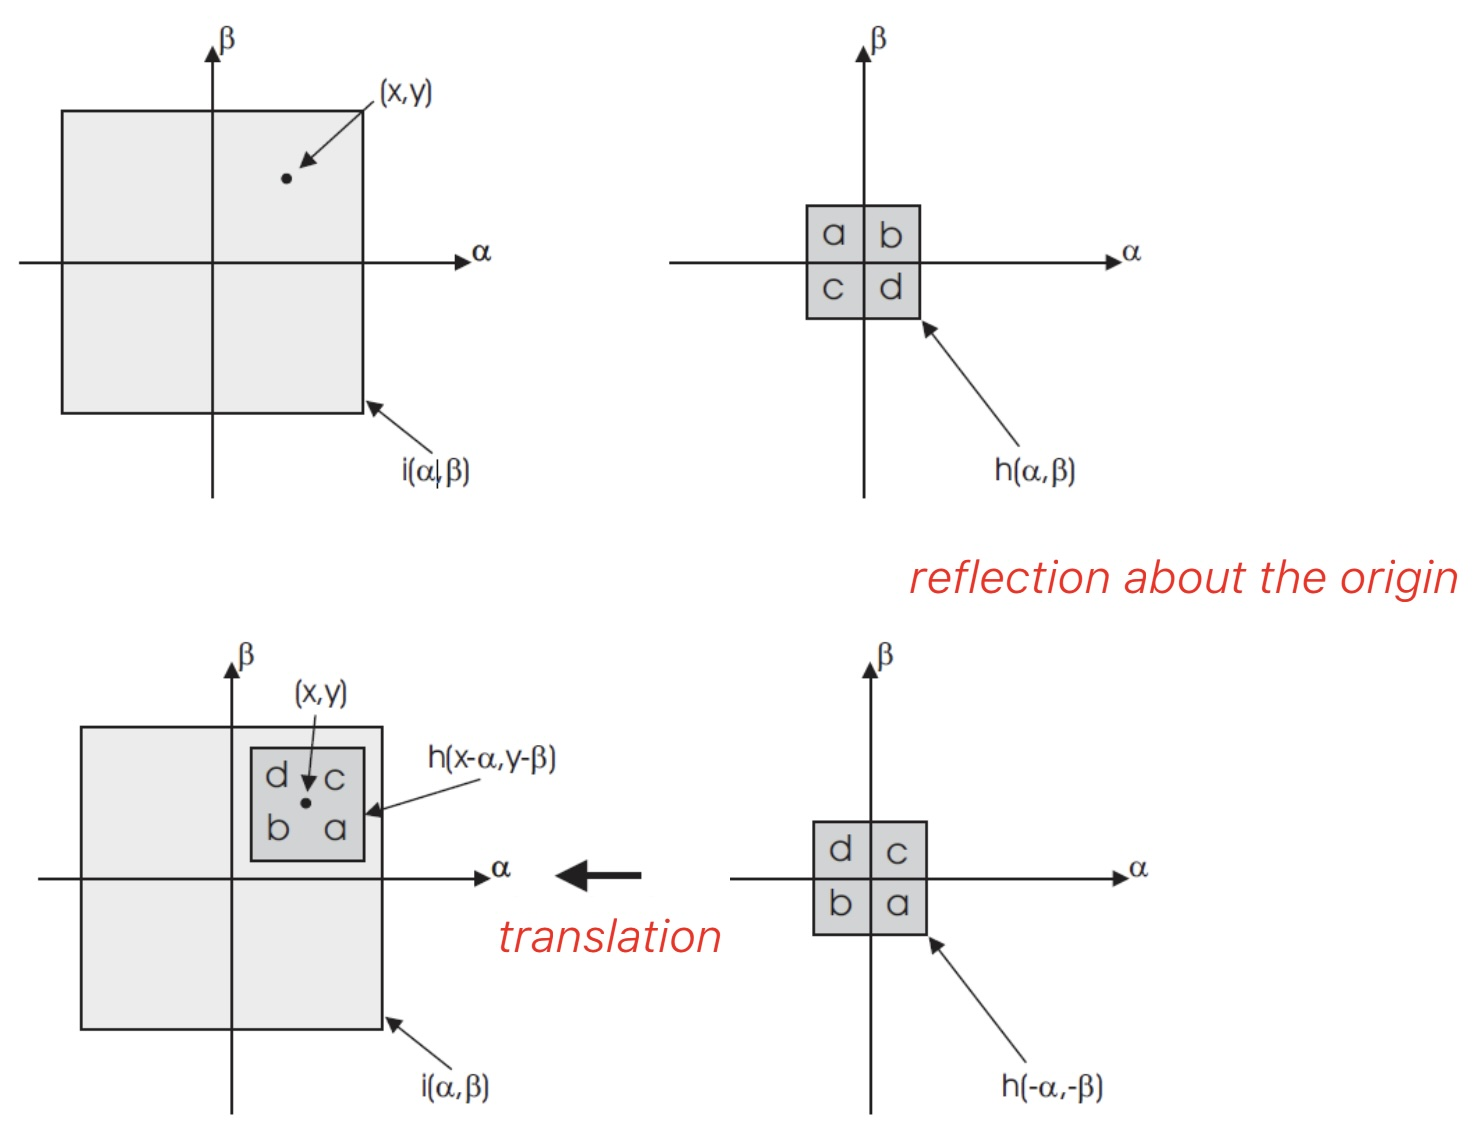
\includegraphics[width=0.6\linewidth]{./img/graphical_convolution.jpg}
  \caption{A graphical view of convolution}
  \label{fig:graphical_convolution}
\end{figure}

Convolutions have some useful properties:
\begin{itemize}
  \item \textbf{Associative property}: $f * (g * h) = (f*g)*h$ (useful because we can decompose kernels and obtain faster operations).
  \item \textbf{Commutative property}: $f*g = g*f$.
  \item \textbf{Distributive property}: $f*(g+h) = f*g + f*h$.
  \item \textbf{Convolution commutes with differentiation}: $(f*g)' = f'*g = f*g'$.
\end{itemize}

The correlation of signal $i(x,y)$  with respect to signal $h(x,y)$ is defined as:
$$i(x,y) \circ h(x,y) = \int_{-\infty}^{\infty} \int_{-\infty}^{\infty} i(\alpha, \beta) h(x+\alpha, y+\beta) \, d\alpha  d\beta $$

Correlation is not commutative, unlike the convolution.

\subsubsection{Discrete convolution}

Normal convolution is useful for signal theory, but we want to have a discrete convolution, where we use summations instead of integrals.
The four convolution properties highlighted for the convolution hold for the discrete one too.

\subsubsection{Practical implementation}
The ``convolution'' operation in many Convolutional Neural Network (CNN) implementations is technically cross-correlation. This is equivalent to classical convolution if the kernel is flipped; the weights learned by the CNN constitute this kernel.

In image processing, both the input image and the kernel are represented as matrices of finite dimensions. The image is typically much larger than the kernel.
To generate the output (often called a feature map), the kernel is slid across the input image. At each position, the dot product between the kernel and the overlapping input region is computed.

A challenge arises at image borders, as the kernel may extend beyond the input matrix boundaries.
Two primary strategies address this:
\begin{itemize}
  \item \texttt{VALID} convolution (cropping): The convolution is computed only for positions where the kernel fully overlaps the input. This approach is common in some image processing contexts.
  \item \texttt{SAME} convolution (padding): The input image is padded before convolution, often with the goal of preserving the spatial dimensions of the input in the output. This is generally preferred in CNNs. Common padding methods include:
    \begin{itemize}
        \item Zero-padding: Adding zeros around the border.
        \item Replication padding: Replicating border pixel values.
        \item Reflection padding: Reflecting pixel values across the border (e.g., reflecting $k$ pixels, where $k$ often corresponds to half the kernel width/height).
    \end{itemize}
\end{itemize}

Without padding (i.e., using \texttt{VALID} convolution), the operation reduces the spatial dimensions of the output.

\begin{figure}[htbp]
  \centering
  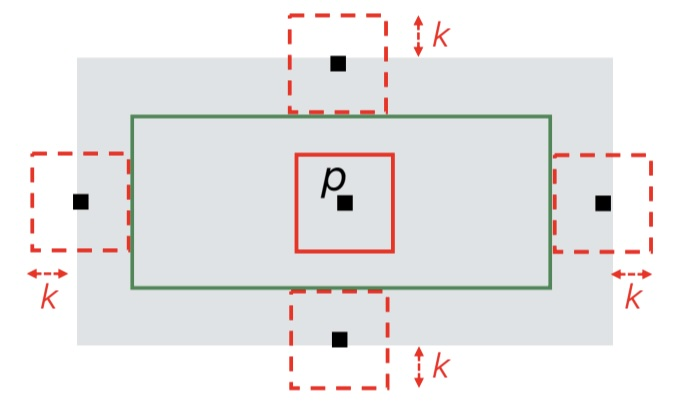
\includegraphics[width=0.55\linewidth]{./img/convolution_visualization.jpg}
  \caption{Convolutions crop the image}
  \label{fig:convolution_visualization}
\end{figure}

\subsubsection{Mean filter}

\textbf{Mean filtering} is the \textbf{simplest and fastest way to denoise an image}.
It consists in replacing each pixel intensity by the \textbf{average intensity over a chosen neighbourhood}.
According to signal processing theory, the Mean Filter carries out a \textbf{low-pass filtering operation}, which in image processing is \textbf{also referred to as image smoothing}.
Smoothing is often aimed at image denoising, but sometimes is used to cancel out small-size unwanted details that might hinder the image analysis task.
Linear filtering \textbf{reduces noise but blurs the image}, so we lose sharpness.

% lecture 3
\subsubsection{Gaussian filter}

The Gaussian filter is an LTE operator whose impulse response is a 2D Gaussian function.

\begin{figure}[htbp]
  \centering
  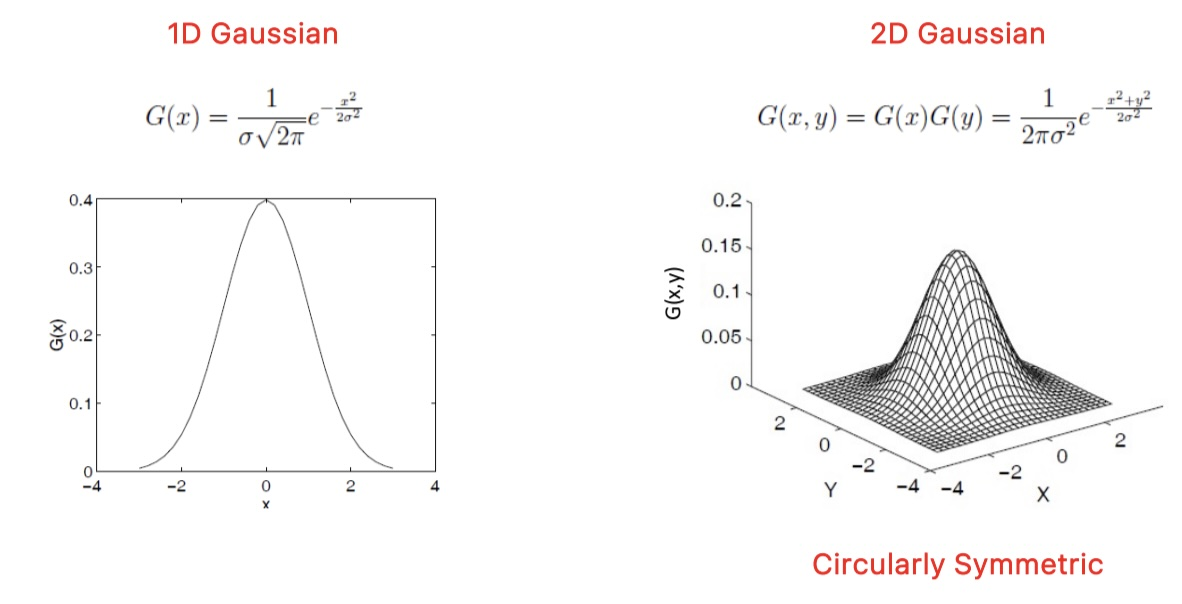
\includegraphics[width=0.7\linewidth]{./img/gaussian_filter.jpg}
  \caption{1D and 2D Gaussian plot}
  \label{fig:gaussian_filter}
\end{figure}

The larger the size of the gaussian kernel, the more accurate the approximation will be, but the computational cost grows with the filter size.
We should then use larger sizes for filters with higher $\sigma$, smaller sizes whenever $\sigma$ is smaller.
A typical rule is to choose the size of the filter by capturing the interval $[-3\sigma, +3\sigma]$ since it captures 99\% of the energy of the Gaussian impulse.

To speedup the filtering we can apply the 2D gaussian by doing 2 1D gaussian filterings.

We also observe that the higher the $\sigma$, the higher is the smoothing caused by the filter.
We can use this filter to remove details from the image.

\subsubsection{Median filter}

There is noise that Gaussian filters can't handle well, that is the \textbf{salt and pepper noise}. It's usually caused by image corruption (or broken pixels in the sensor).
On this noise linear filtering is ineffective, and just blurs the image.

We can use a \textbf{non-linear filter}, where each pixel intensity is replaced by the \textbf{median over a given neighbourhood}.
Median filtering counteracts impulse noise effectively, since \textbf{outliers tend to fall at either the top or the bottom end of the sorted intensities}.
Median filtering tends to keep sharper edges than linear filters such as the Mean or the Gaussian.

\begin{figure}[htbp]
  \centering
  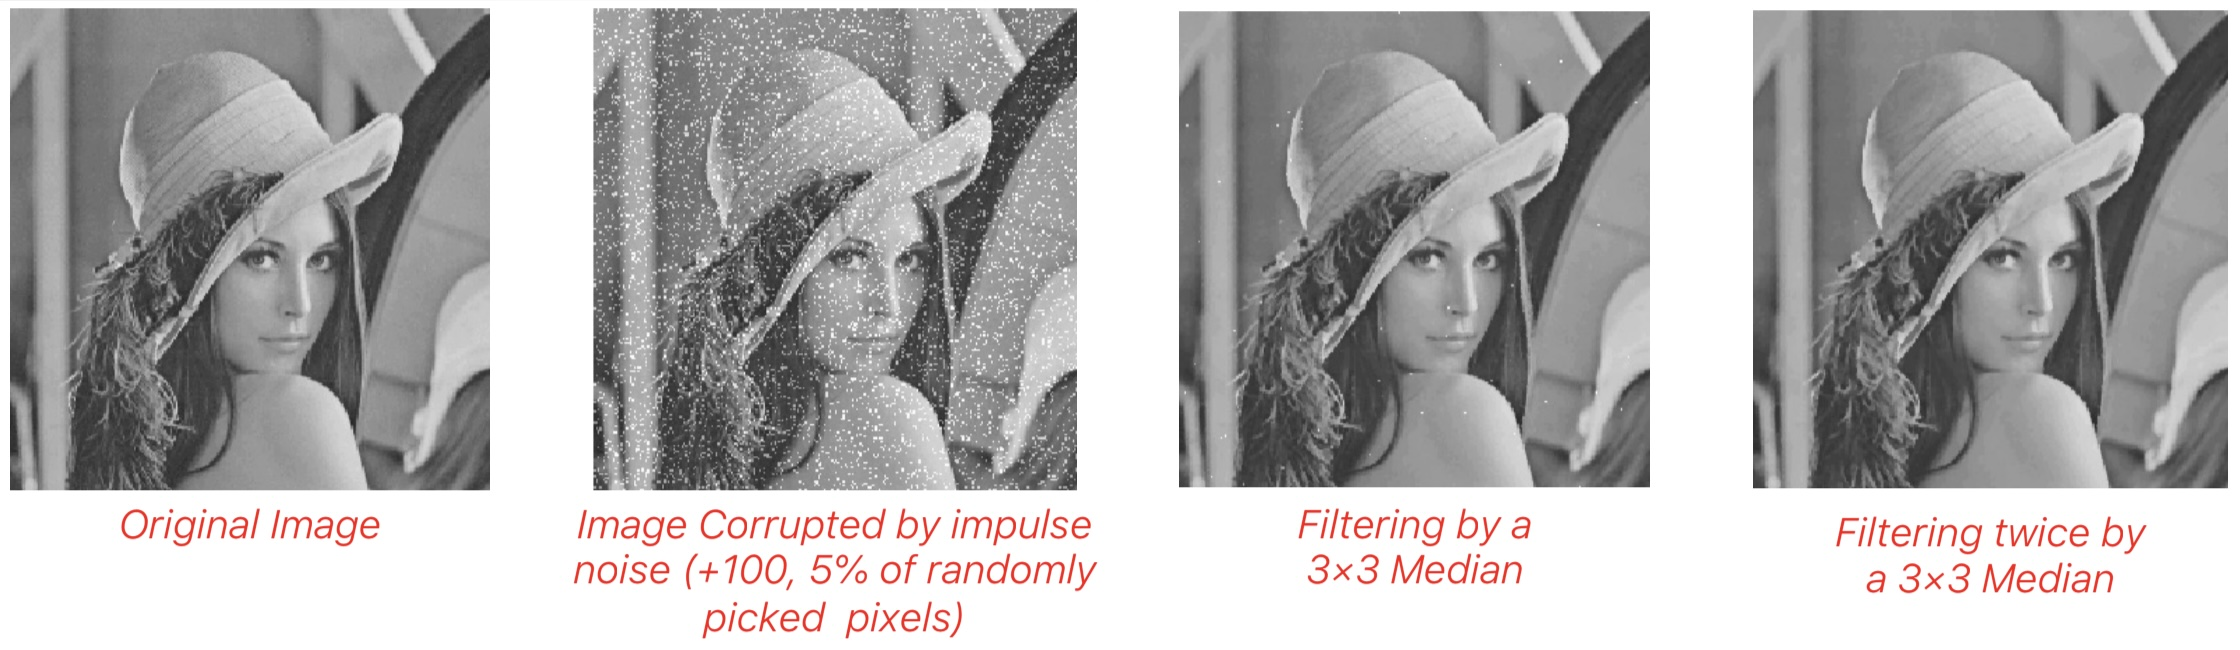
\includegraphics[width=0.9\linewidth]{./img/median_filter_application.jpg}
  \caption{Example of the power of the median filter}
  \label{fig:median_filter_application}
\end{figure}

The median filter can effectively denoise the image without introducing significant blur, yet, Gaussian-like noise, such as sensor noise, cannot be dealt with by the median, as this would require computing new noiseless intensities.

\subsubsection{Bilateral filter}
The \textbf{bilateral filter} is a non-linear filter that \textbf{preserves edges} while reducing noise, such as Gaussian-like noise. This characteristic, also known as edge-preserving smoothing, allows it to denoise images without significantly blurring sharp features.

\begin{figure}[htbp]
  \centering
  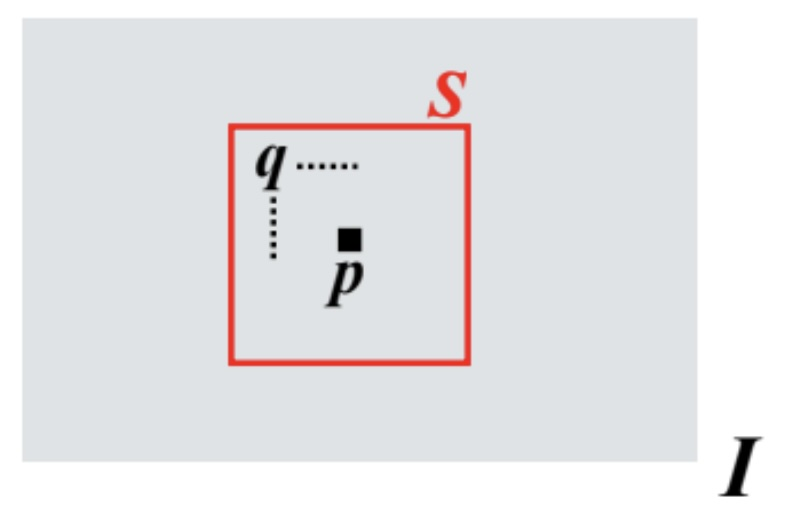
\includegraphics[width=0.5\linewidth]{./img/bilateral_filter_application.jpg}
  \caption{Application of the bilateral filter}
  \label{fig:bilateral_filter_application}
\end{figure}

The filtered output $O(p)$ for a pixel $p$ is computed as a weighted average of neighboring pixel intensities:
\begin{align*}
O(p) &= \sum_{q \in S} H(p,q) \cdot I_q \\
\intertext{where $S$ is the set of pixels in the neighborhood of $p$, $I_q$ is the intensity of pixel $q$, and the weight $H(p,q)$ is given by:}
H(p,q) &= \frac{1}{W(p)} G_{\sigma_s}(d_s(p,q)) \, G_{\sigma_r}(d_r(I_p, I_q))
\end{align*}
Here, $G_{\sigma_s}$ and $G_{\sigma_r}$ are Gaussian functions. The components are:
\begin{itemize}
  \item \textbf{Spatial distance}: $d_s(p,q) = ||p-q||_2 = \sqrt{(u_p - u_q)^2 + (v_p - v_q)^2}$, where $(u_p, v_p)$ are the coordinates of pixel $p$. This term penalizes distance in space.
  \item \textbf{Range (intensity) distance}: $d_r(I_p, I_q) = |I_p - I_q|$. This term penalizes differences in pixel intensities.
  \item \textbf{Normalization factor}: $W(p) = \sum_{q \in S} G_{\sigma_s}(d_s(p,q)) \, G_{\sigma_r}(d_r(I_p, I_q))$, ensuring that the weights $H(p,q)$ for a given $p$ sum to 1.
\end{itemize}

Within the support neighborhood $S$, a neighboring pixel $q$ is assigned a higher weight $H(p,q)$ if it is both spatially close to $p$ (small $d_s(p,q)$) and has an intensity $I_q$ similar to $I_p$ (small $d_r(I_p,I_q)$).

For a pixel $p$ near an edge, neighboring pixels $q$ on the other side of the edge will have markedly different intensities ($I_q$ vs $I_p$). This results in a large range distance $d_r(I_p,I_q)$, significantly reducing the value of the range Gaussian $G_{\sigma_r}$ and thus the overall weight $H(p,q)$. Consequently, these differing pixels contribute minimally to the output $O(p)$, thereby preserving the edge.

A key characteristic is that \textbf{the filter weights $H(p,q)$ must be recomputed for each pixel $p$}, as they depend on the local image content (specifically, $I_p$).

\begin{figure}[htbp]
  \centering
  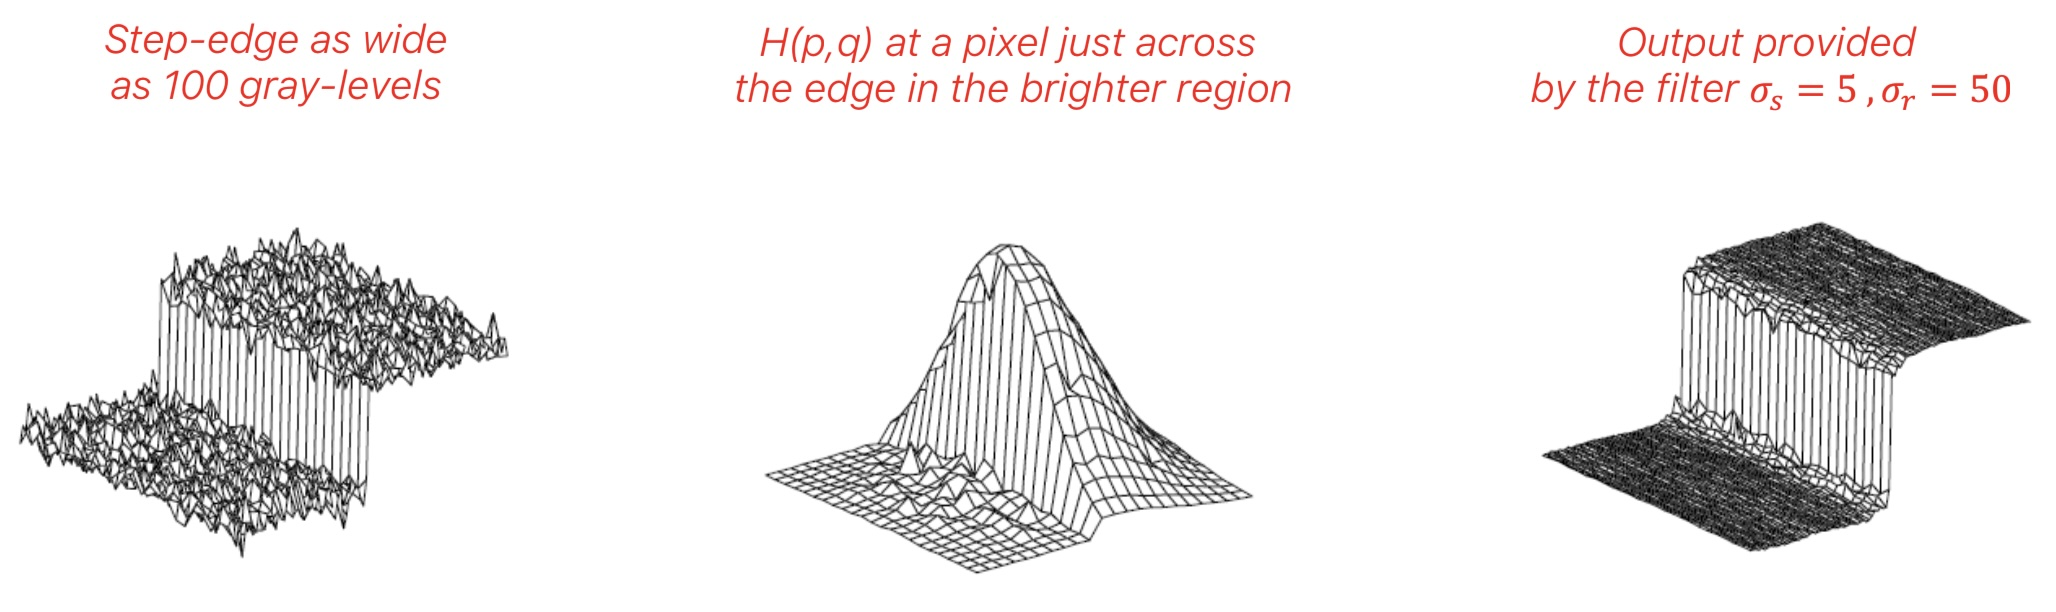
\includegraphics[width=0.9\linewidth]{./img/bilateral_filter.jpg}
  \caption{Bilateral filter applied on an edge}
  \label{fig:bilateral_filter}
\end{figure}

The bilateral filter is almost like a Gaussian filter, except that the Gaussian is modulated by a function that computes the similarity between the central pixel (where the filter is applied) and a pixel in its neighborhood (that is used in blurring).

\begin{itemize}
  \item If the two pixel values are very close, it multiplies the Gaussian coefficient by something close to 1, and hence it is equivalent to Gaussian filtering.
  \item If the pixel values are very different , it will multiply the Gaussian coefficient by a number close to 0, thus turning off the Gaussian filtering for this pixel.
\end{itemize}

Intuitively, this behaviour yields the following result: Gaussian filtering in uniform areas of the image, no filtering across object borders. The bilateral filter will produce a more pleasant results, because it will avoid the introduction of blur between objects while still removing noise in uniform areas

\subsubsection{Non-local means filter}

It's another non-linear edge preserving smoothing filter.
The key idea is that the \textbf{similarity among patches spread over the image} can be deployed to achieve denoising.
It's even more expensive than the bilateral filter, since it has to look at more of the image.

\begin{figure}[htbp]
  \centering
  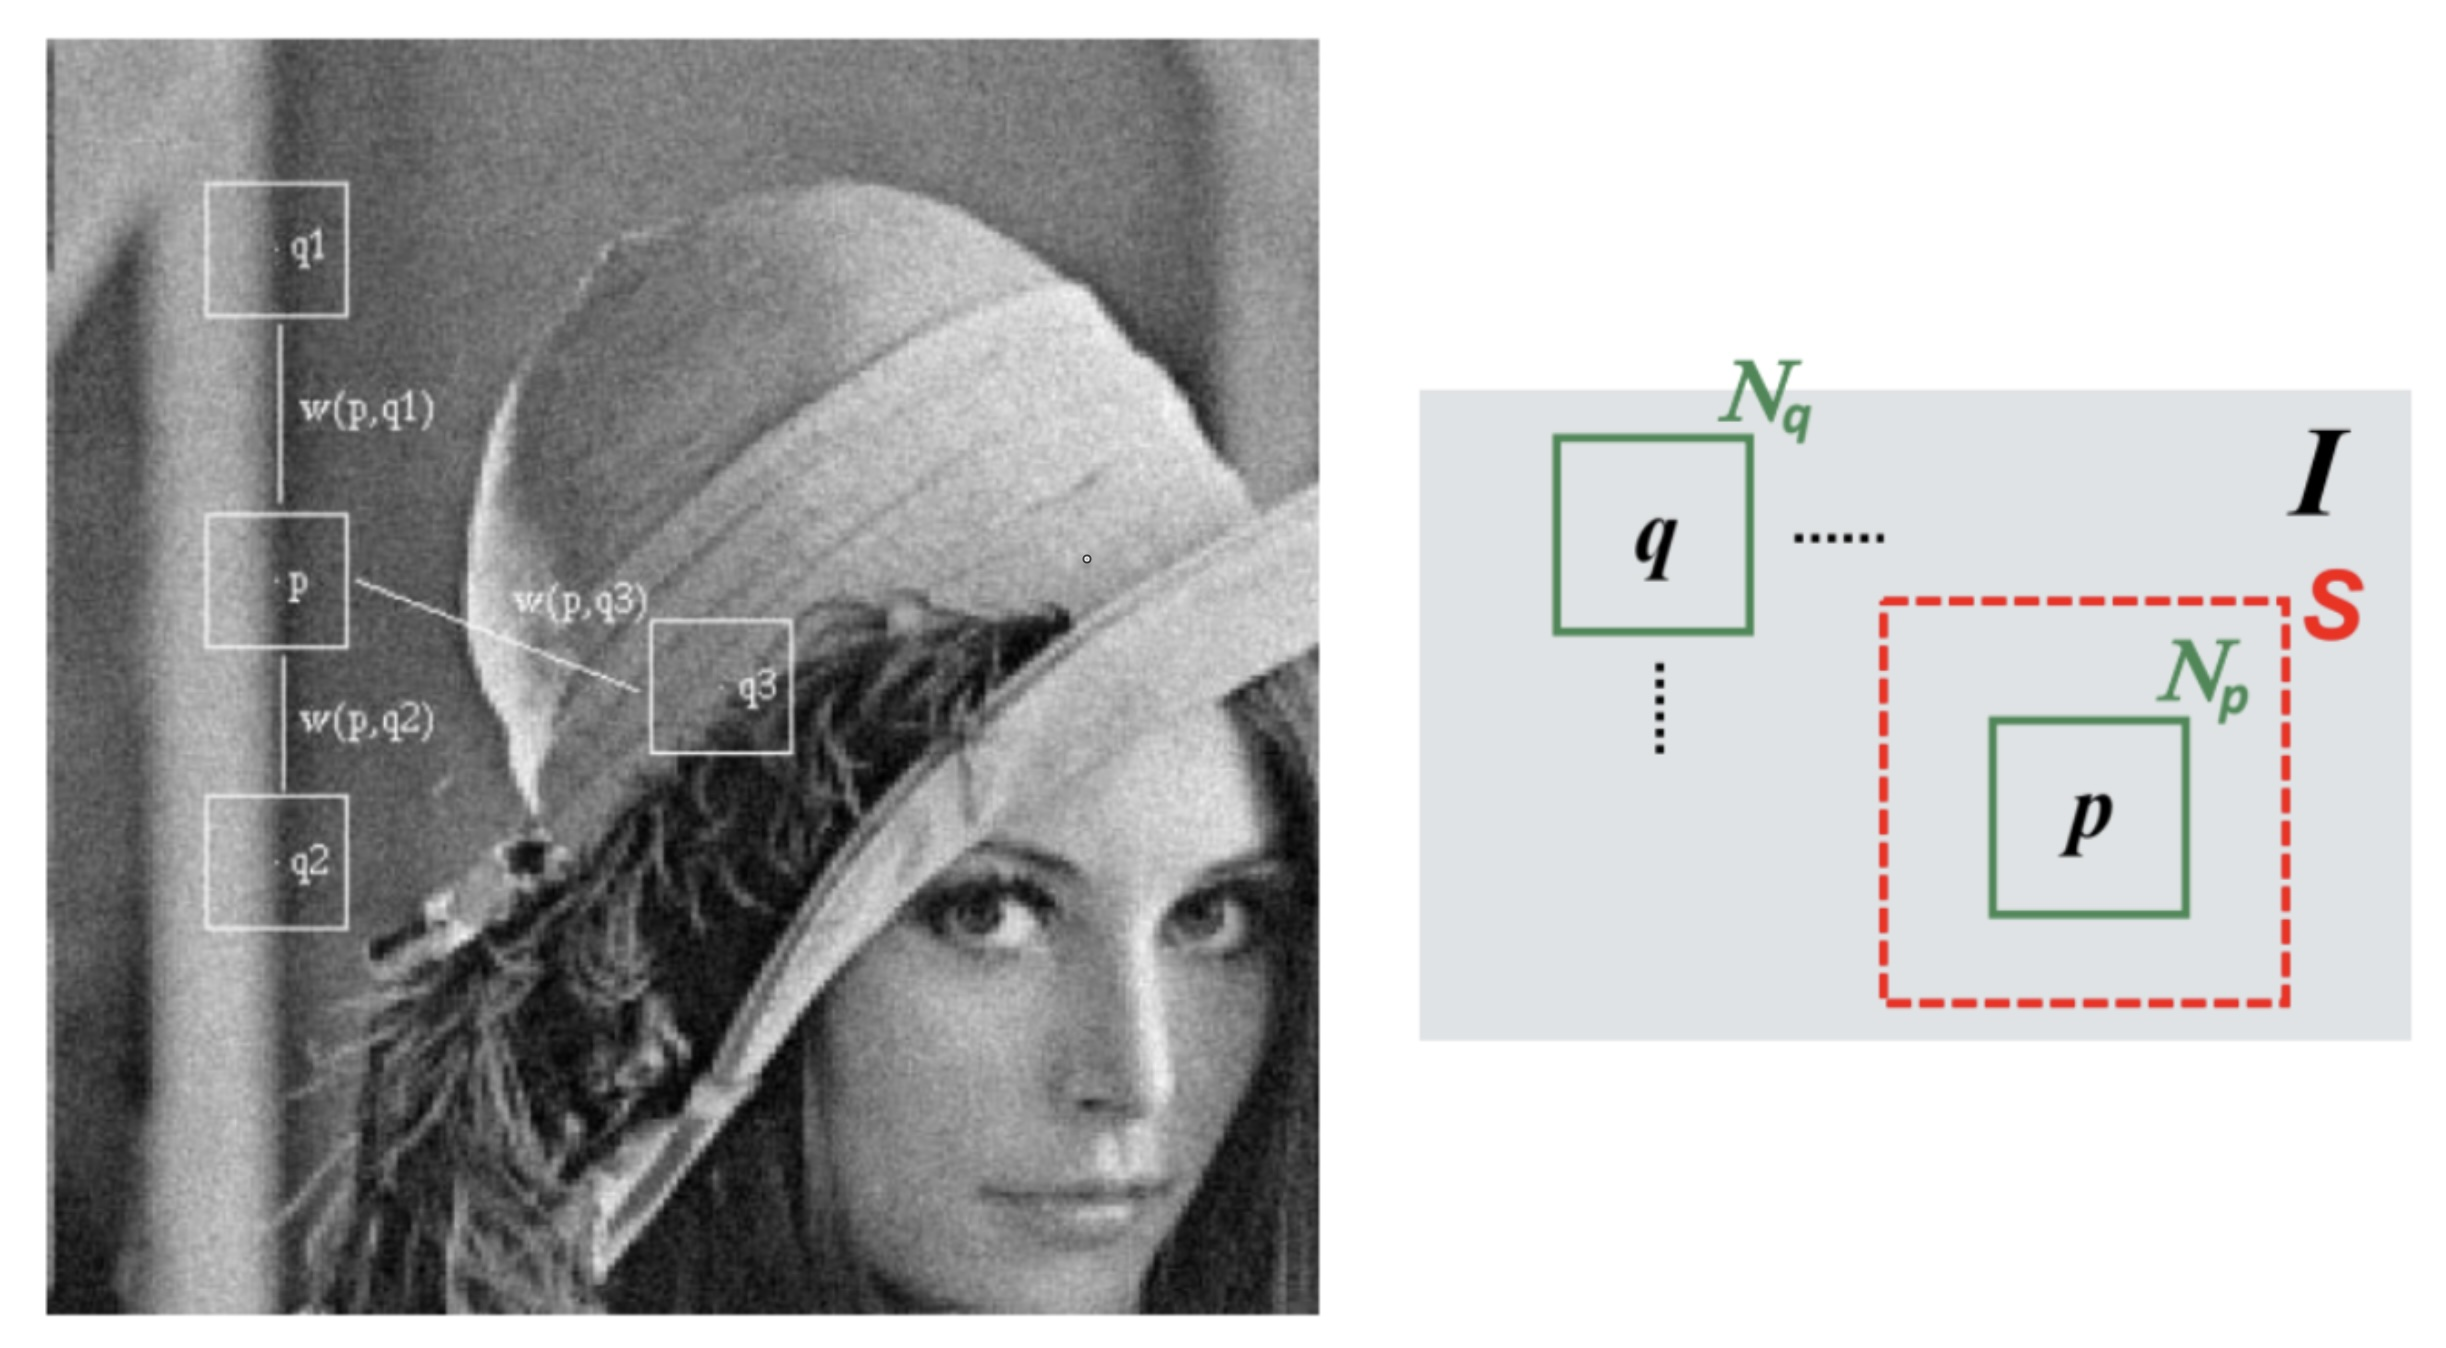
\includegraphics[width=0.7\linewidth]{./img/nonlocalmeans_filter.jpg}
  \caption{Non-local means filter}
  \label{fig:nonlocalmeans_filter}
\end{figure}

\begin{figure}[htbp]
  \centering
  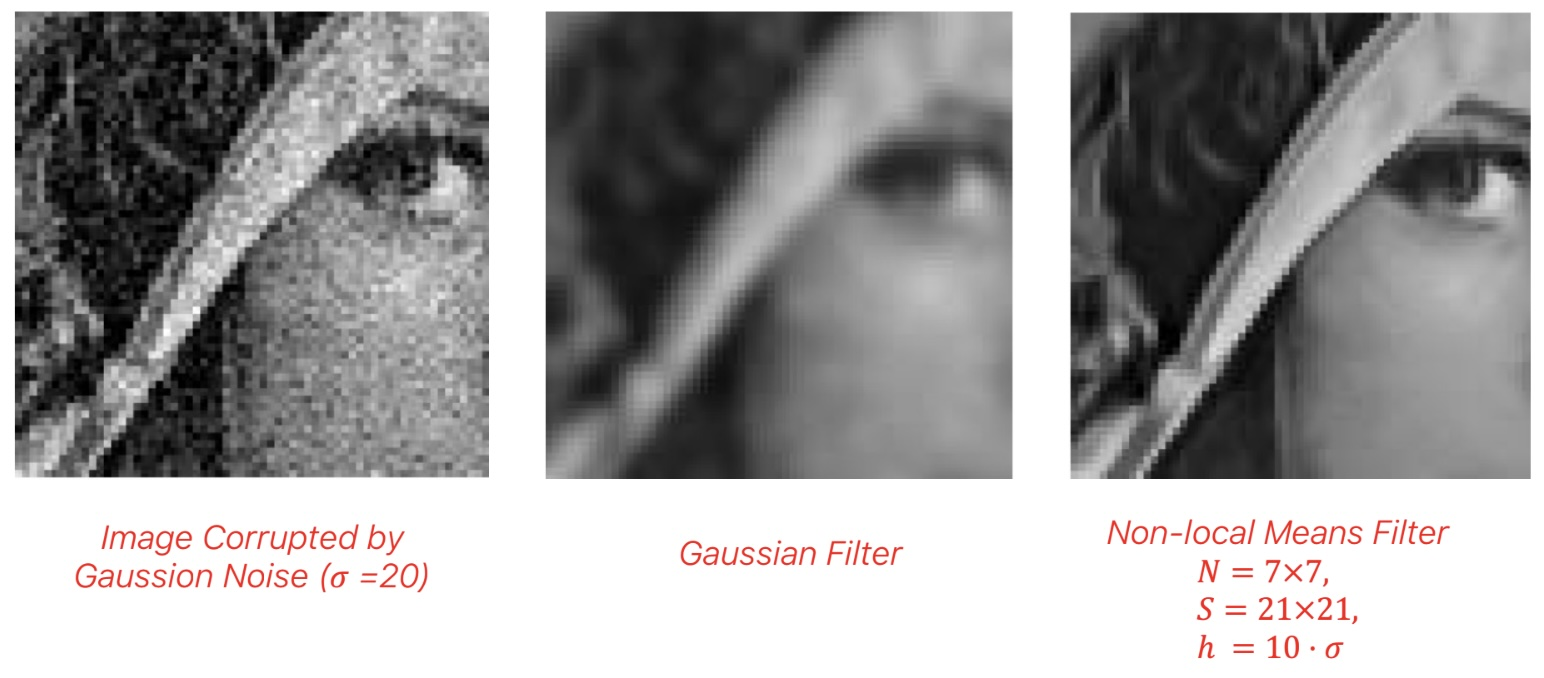
\includegraphics[width=0.7\linewidth]{./img/nonlocalmeans_comparison.jpg}
  \caption{Difference between Gaussian filter and non-local means filter}
  \label{fig:nonlocalmeans_comparison}
\end{figure}

\subsection{Edge detection}

Edge points are local image features representing significant discontinuities in intensity. They often correspond to object boundaries or changes in surface properties, thus capturing important semantic information. Edges typically occur in transition zones between regions of differing intensities.

\paragraph{1D step-edge}
In a 1D signal, an edge (or step-edge) manifests as a sharp change in intensity.
A basic detection method involves thresholding the absolute value of the signal's first derivative.

\paragraph{2D step-edge}
A 2D step-edge is characterized by its strength (magnitude) and its orientation. The gradient vector,
\[ \nabla I(x,y) = \frac{\partial I(x,y)}{\partial x}\mathbf{i} + \frac{\partial I(x,y)}{\partial y}\mathbf{j} \]
points in the \textbf{direction of maximum intensity variation}. In discrete images, partial derivatives are approximated using finite differences (yielding $I_x$ and $I_y$).
The gradient magnitude, indicating edge strength, can be estimated using various approximations. For example, $|\nabla I| \approx \max(|I_x|, |I_y|)$ is computationally efficient but not perfectly rotationally invariant.

\paragraph{Edges and noise}
Real-world images contain noise, which can cause edges to appear irregular. Computing derivatives on noisy signals is an ill-posed problem because \textbf{derivatives tend to amplify high-frequency noise}.
To improve robustness, images are often smoothed before differentiation. However, this smoothing also blurs true edges, which can reduce their apparent strength and make precise localization more challenging, as distinct pixel intensities in the original image are averaged.

\paragraph{Prewitt and Sobel}
The Prewitt and Sobel operators address edge detection in noisy images by convolving the image with small ($3 \times 3$) kernels that combine smoothing and differentiation.
Each operator uses a pair of kernels: one to estimate the gradient component $G_x$ (approximating $I_x$, responsive to vertical edges) and another for $G_y$ (approximating $I_y$, responsive to horizontal edges). Each kernel effectively smooths the image in one direction and computes the derivative in the perpendicular direction.
After convolving the image with both kernels to obtain $G_x$ and $G_y$, the gradient magnitude and direction are computed:
\begin{align*}
\text{Magnitude} &= \sqrt{G_x^2 + G_y^2} \\
\text{Direction} &= \arctan^2(\frac{G_y}{G_x})
\end{align*}
The Sobel operator gives more weight to the central pixels in its smoothing component, generally offering better noise suppression than the Prewitt operator, which uses uniform weights. This can come at the cost of slightly more edge blurring for Sobel.

\subsubsection{Non-Maxima Suppression (NMS)}

Detecting edges by simply thresholding the gradient magnitude often produces thick or inaccurate edges, partly because \textbf{it is difficult to choose a single, globally optimal threshold}.
Non-Maxima Suppression (NMS) is a technique to thin wide edges into sharper lines by selecting only pixels that are local maxima of the gradient magnitude.
For 2D images, NMS involves:
\begin{itemize}
  \item Identifying local maxima of the gradient magnitude.
  \item This search for maxima is performed along the gradient direction at each pixel (which is orthogonal to the potential edge direction).
\end{itemize}
Since the true gradient direction (estimated locally) may not align perfectly with the discrete pixel grid, gradient magnitudes at sub-pixel locations along this direction are typically estimated using interpolation (e.g., linear interpolation) from neighboring grid pixels.
A final thresholding step is often applied to the NMS output. This helps to prune weak edges that might arise from noise or less significant image details, even after suppression.

\subsubsection{Canny's edge detector}
Canny formulated quantitative criteria for evaluating edge detector performance and sought an optimal filter based on these:
\begin{itemize}
  \item \textbf{Good detection}: High probability of detecting true edges and low probability of falsely detecting non-edges (robustness to noise).
  \item \textbf{Good localization}: Detected edges should be as close as possible to the true edges.
  \item \textbf{Single response}: The detector should return only one point for each true edge (minimizing multiple responses to a single edge).
\end{itemize}

The Canny edge detection algorithm typically involves the following steps:
\begin{enumerate}
  \item \textbf{Gaussian smoothing}: Reduce noise using a Gaussian filter. The 2D Gaussian convolution $G(x,y) = G(x)G(y)$ is separable, allowing for efficient computation as two 1D convolutions.
  \item \textbf{Gradient computation}: Calculate gradient magnitude and direction (e.g., using Sobel operators).
  \item \textbf{Non-Maxima Suppression (NMS)}: Thin wide ridges of gradient magnitude into sharp lines by preserving only pixels that are local maxima along the gradient direction.
  \item \textbf{Hysteresis thresholding}: This step addresses the issue of "edge streaking" (where an edge contour is broken if its gradient magnitude locally dips below a single threshold). It uses two thresholds: a high threshold $T_H$ and a low threshold $T_L$.
    \begin{itemize}
      \item Pixels with gradient magnitude above $T_H$ are immediately classified as "strong" edge pixels.
      \item Pixels with gradient magnitude between $T_L$ and $T_H$ are classified as "weak" edge pixels.
      \item Pixels with gradient magnitude below $T_L$ are suppressed.
    \end{itemize}
    Strong edge pixels are kept. Weak edge pixels are kept only if they are connected to a strong edge pixel (directly or via other connected weak edge pixels). This connectivity check is often implemented by tracking along contours from strong edge pixels.
\end{enumerate}

\paragraph{Zero-crossing of the second derivative}
An alternative to finding peaks in the first derivative (gradient magnitude) is to locate edges at the zero-crossings of the second derivative of the signal. This approach can offer precise localization but generally involves more computation due to the calculation of second-order derivatives, which are also more sensitive to noise.

\subsubsection{Second derivative along the gradient \& Laplacian}
The second derivative along the gradient's direction, $n^T H n$, can be used to find edge locations.
\begin{itemize}
  \item $n = \frac{\nabla I(x,y)}{||\nabla I(x,y)||}$ is the unit vector in the gradient's direction.
  \item $H =  \begin{bmatrix} \frac{\partial^2 I(x,y)}{\partial x^2} & \frac{\partial^2 I(x,y)}{\partial x \partial y} \\ \frac{\partial^2 I(x,y)}{\partial y \partial x} & \frac{\partial^2 I(x,y)}{\partial y^2} \end{bmatrix} $ is the Hessian matrix.
\end{itemize}
Computing this directional second derivative explicitly is computationally expensive.

\paragraph{Discrete Laplacian}
The Laplacian operator, $\nabla^2 I = I_{xx} + I_{yy}$, is a scalar quantity that is rotationally invariant. Its zero-crossings often occur close to the zero-crossings of the second derivative along the gradient direction. Approximating derivatives with finite differences allows for a discrete Laplacian filter, which is much faster to compute than the directional second derivative.

\subsubsection{Laplacian of Gaussian (LoG)}
To combine noise reduction with second-derivative edge detection, the Laplacian of Gaussian (LoG) operator is used. The process is:
\begin{enumerate}
  \item \textbf{Gaussian smoothing}: Convolve the image $I(x,y)$ with a Gaussian kernel $G(x,y)$ to get $\tilde{I}(x,y) = I(x,y) * G(x,y)$.
  \item \textbf{Laplacian operation}: Compute the Laplacian of the smoothed image, $\nabla^2 \tilde{I}(x,y)$.
  \item \textbf{Zero-crossing detection}: Identify pixels where the $\nabla^2 \tilde{I}(x,y)$ value changes sign. These zero-crossings indicate potential edges.
\end{enumerate}
Due to the linearity of convolution and differentiation, $\nabla^2 (I * G) = I * (\nabla^2 G)$. Thus, one can convolve the image directly with a pre-computed LoG kernel ($\nabla^2 G$), improving efficiency.

When a sign change (zero-crossing) is detected between adjacent pixels, the edge can be localized more precisely:
\begin{itemize}
  \item At the pixel with the positive LoG value (typically corresponding to the darker side of an intensity step).
  \item At the pixel with the negative LoG value (brighter side).
  \item At the pixel whose LoG value has the \textbf{smallest absolute magnitude} among the pair straddling the zero-crossing. This is often preferred as it places the edge closer to the true zero-crossing point.
\end{itemize}
A larger $\sigma$ for the Gaussian component results in more smoothing, detecting larger scale edges while suppressing finer details and noise. This is beneficial for noisy images.

\begin{figure}[htbp]
  \centering
  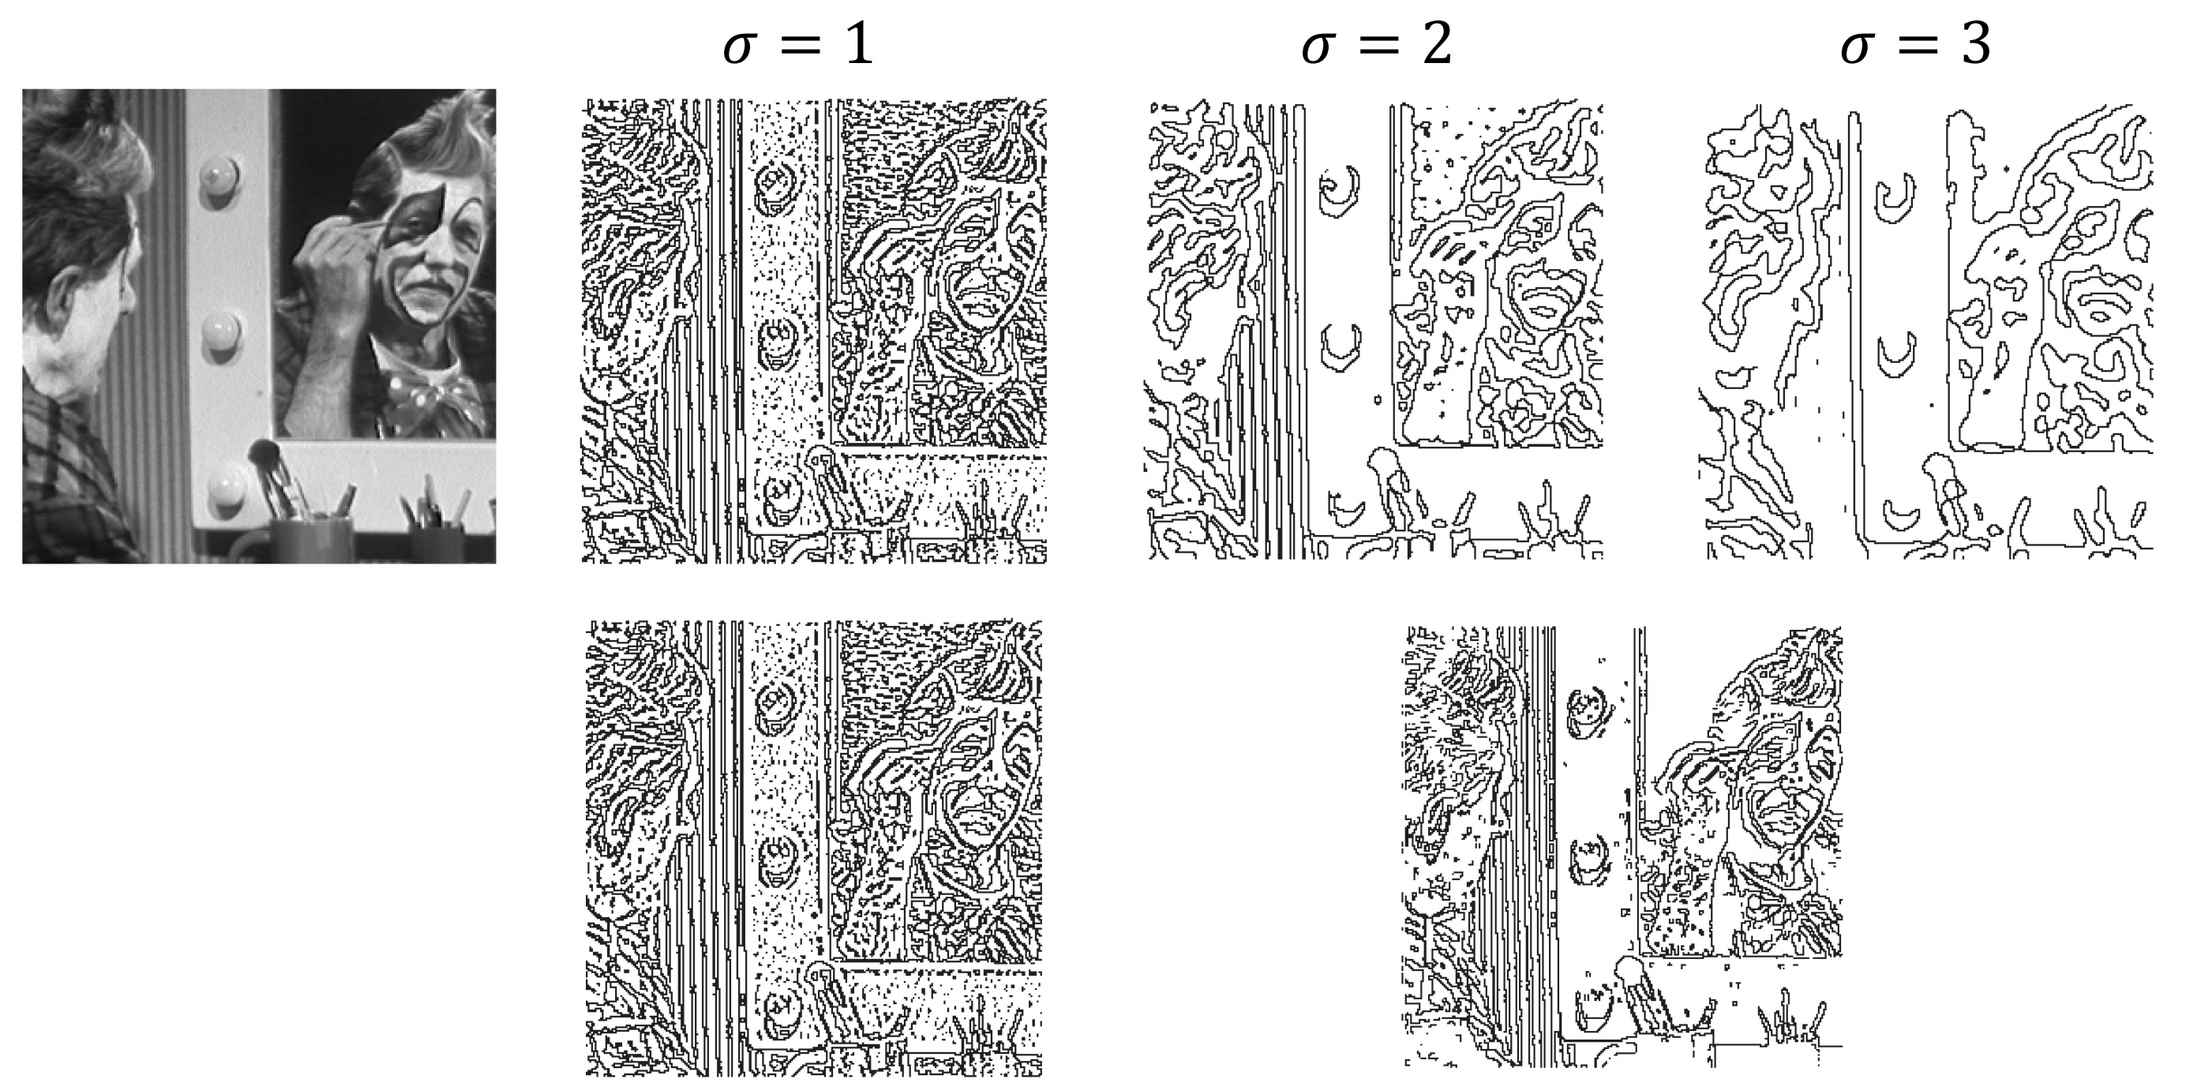
\includegraphics[width=0.7\linewidth]{./img/log_application.jpg}
  \caption{Examples of LoG application}
  \label{fig:log_application}
\end{figure}

\subsection{Feature detection and matching}
Feature detection and matching are fundamental for various computer vision tasks, such as image stitching, 3D reconstruction, object recognition, and tracking. The core idea is to identify distinctive points (features) in one image and find their counterparts in other images of the same scene or object.
These corresponding image points are projections of the same 3D point viewed from different perspectives. Establishing these correspondences can be challenging because the appearance of points can vary significantly across different views due to changes in viewpoint, illumination, scale, and other factors.

\subsubsection{Local invariant features paradigm}
The task of establishing correspondences using local features is typically broken down into three steps:
\begin{itemize}
  \item \textbf{Detection}: Identify salient interest points (keypoints) in the image.
  \item \textbf{Description}: Compute a feature descriptor for the local image region around each keypoint. This descriptor numerically captures the appearance of the neighborhood.
  \item \textbf{Matching}: Compare descriptors from different images to find pairs that are most similar, thereby establishing correspondences.
\end{itemize}
Ideally, descriptors should be \textbf{invariant} (or at least robust) to transformations such as changes in scale, rotation, illumination, and viewpoint.

\subsubsection{Properties of good detectors/descriptors}
\begin{itemize}
  \item \textbf{Detector criteria}:
  \begin{itemize}
    \item Repeatability: The detector should consistently find the same keypoints in different images of the same scene, despite transformations.
    \item Saliency (or distinctiveness): Keypoints should be located in textured regions with informative patterns, making them distinguishable.
  \end{itemize}
  \item \textbf{Descriptor criteria}:
  \begin{itemize}
    \item Distinctiveness: The descriptor for one keypoint should be significantly different from descriptors of other, unrelated keypoints.
    \item Robustness (or invariance): The descriptor for a specific keypoint should remain similar even when the keypoint is viewed under different conditions (e.g., illumination changes, small viewpoint variations). There's often a trade-off between distinctiveness and robustness.
    \item Compactness: The descriptor should be as concise as possible to reduce storage and computational cost for matching.
    \item Efficiency: Computation of descriptors should be fast.
  \end{itemize}
\end{itemize}
Overall efficiency is crucial for both detection and description, especially for detectors that operate on the entire image. Descriptors are computed only at detected keypoints.

Edge pixels, while indicative of intensity changes, often suffer from local ambiguity: a small patch centered on an edge looks very similar to patches at nearby points along the same edge (the aperture problem). This makes it difficult to uniquely localize or match edge pixels based solely on their immediate neighborhood.

\subsubsection{Moravec Interest Point Detector}
The Moravec detector identifies interest points by evaluating how dissimilar a local image patch is from slightly shifted versions of itself. The "cornerness" $C(p)$ at a pixel $p$ is defined as the minimum sum of squared differences (SSD) between an image patch $N(p)$ centered at $p$ and patches $N(q)$ centered at its 8 immediate neighbors $q \in n_8(p)$:
\[ C(p) = \min_{q \in n_8(p)} \sum_{(u,v) \in \text{Patch}} (N_p(u,v) - N_q(u,v))^2 \]
where $N_p(u,v)$ is the intensity of a pixel at relative coordinates $(u,v)$ within the patch centered at $p$.
After computing $C(p)$ for all pixels, potential interest points are those where $C(p)$ exceeds a threshold, followed by Non-Maxima Suppression (NMS) to select only local peaks.

\begin{figure}[htbp]
  \centering
  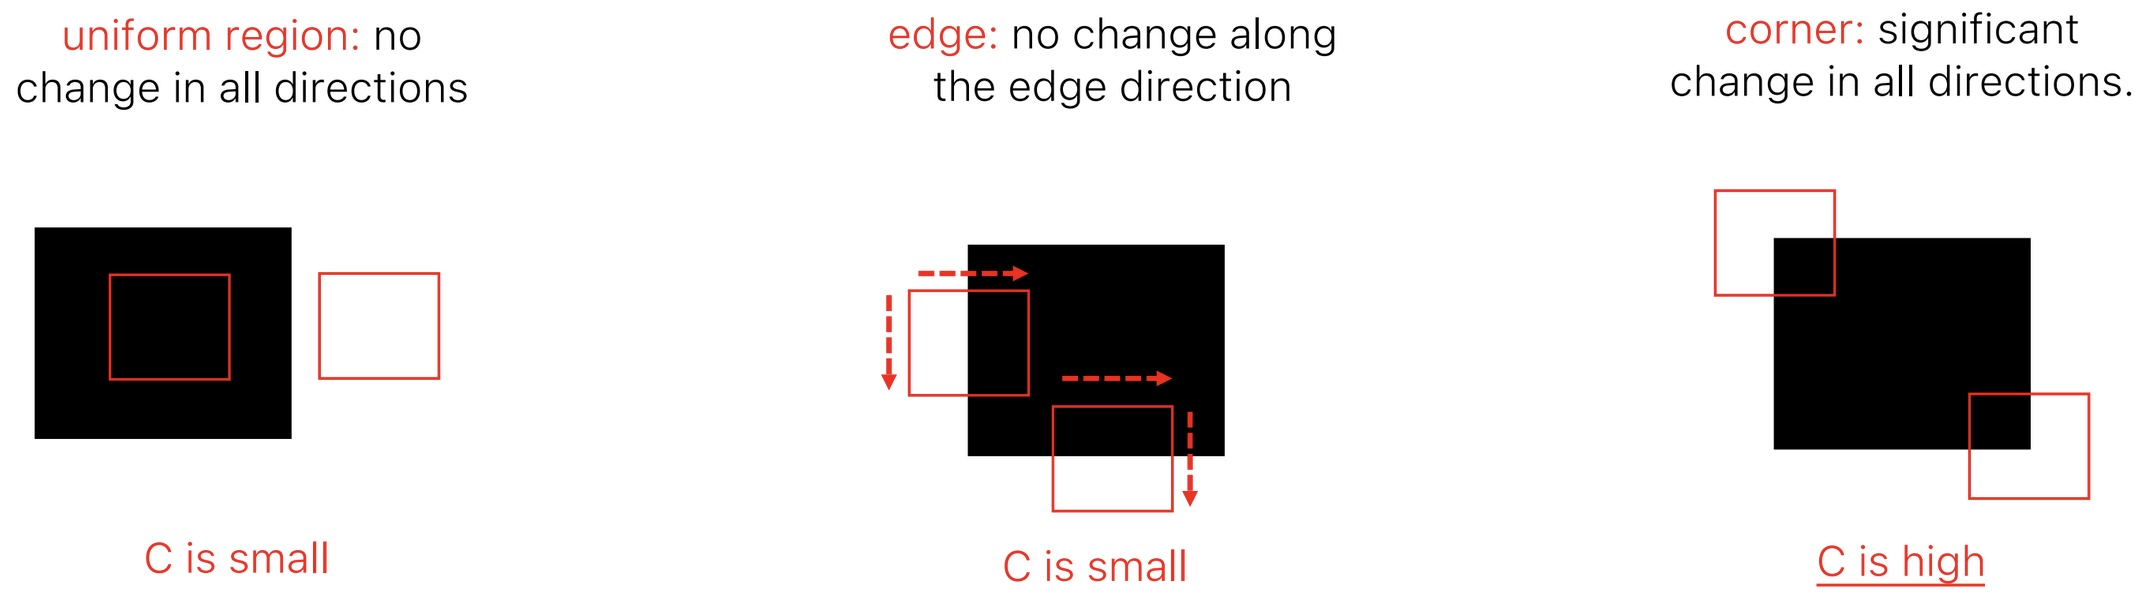
\includegraphics[width=0.9\linewidth]{./img/cornerness.jpg}
  \caption{Illustration of patch shifts for cornerness evaluation. A corner (right) shows significant intensity changes in all shift directions. An edge (middle) shows little change along the edge direction. A flat region (left) shows little change in any direction.}
  \label{fig:cornerness}
\end{figure}

\subsubsection{Harris Corner Detector}
Harris and Stephens refined Moravec's idea by considering infinitesimal shifts $(\Delta x, \Delta y)$ and analyzing the local image structure using a continuous formulation. The sum of squared differences $E(\Delta x, \Delta y)$ for a shift $(\Delta x, \Delta y)$ over a window $w(u,v)$ centered at $(x_0, y_0)$ is:
\[ E(\Delta x, \Delta y) = \sum_{u,v} w(u,v) [I(x_0+u+\Delta x, y_0+v+\Delta y) - I(x_0+u, y_0+v)]^2 \]
Using a first-order Taylor expansion for the intensity difference:
\[ I(x_0+u+\Delta x, y_0+v+\Delta y) - I(x_0+u, y_0+v) \approx I_x(x_0+u, y_0+v)\Delta x + I_y(x_0+u, y_0+v)\Delta y \]
where $I_x$ and $I_y$ are partial derivatives of the image intensity $I$.
Substituting this into $E(\Delta x, \Delta y)$ yields a quadratic approximation:
\[ E(\Delta x, \Delta y) \approx \begin{bmatrix} \Delta x & \Delta y \end{bmatrix} M \begin{bmatrix} \Delta x \\ \Delta y \end{bmatrix} \]
The matrix $M$, often called the structure tensor or second-moment matrix, is computed for the window around $(x_0,y_0)$:
\[ M = \sum_{u,v} w(u,v)
\begin{bmatrix}
I_x(x_0+u,y_0+v)^2 & I_x(x_0+u,y_0+v)I_y(x_0+u,y_0+v) \\
I_x(x_0+u,y_0+v)I_y(x_0+u,y_0+v) & I_y(x_0+u,y_0+v)^2
\end{bmatrix} \]
The window function $w(u,v)$ is typically a Gaussian or a rectangular window, weighting pixels within the patch.

\begin{figure}[htbp]
  \centering
  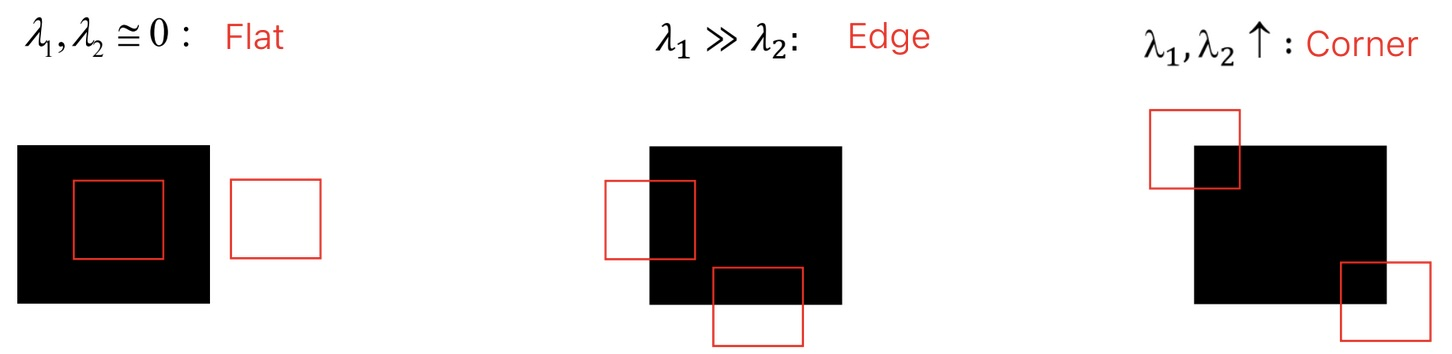
\includegraphics[width=0.9\linewidth]{./img/harris_corner_detector.jpg}
  \caption{Interpretation of eigenvalues ($\lambda_1, \lambda_2$) of matrix $M$ for Harris corner detection. Corners have two large eigenvalues. Edges have one large and one small eigenvalue. Flat regions have two small eigenvalues.}
  \label{fig:harris_corner_detector}
\end{figure}

The matrix $M$ is real and symmetric, so it can be diagonalized by an orthogonal matrix $R$:
\[ M = R\begin{bmatrix} \lambda_1 & 0 \\ 0 & \lambda_2 \end{bmatrix}R^T \]
where $\lambda_1, \lambda_2$ are the eigenvalues of $M$, and the columns of $R$ are the corresponding orthonormal eigenvectors. These eigenvalues characterize the local image structure:
\begin{itemize}
    \item Flat region: $\lambda_1 \approx 0, \lambda_2 \approx 0$. $E(\Delta x, \Delta y)$ is small for all shifts.
    \item Edge: $\lambda_1 \gg 0, \lambda_2 \approx 0$ (or vice versa). $E(\Delta x, \Delta y)$ is large for shifts perpendicular to the edge, small for shifts along the edge.
    \item Corner: $\lambda_1 \gg 0, \lambda_2 \gg 0$. $E(\Delta x, \Delta y)$ is large for shifts in all directions.
\end{itemize}
Explicitly computing eigenvalues at each pixel is computationally intensive. Harris proposed a corner response function $C_H$:
\[ C_H = \det(M) - k (\text{trace}(M))^2 = \lambda_1 \lambda_2 - k (\lambda_1 + \lambda_2)^2 \]
where $k$ is an empirical constant (e.g., $0.04-0.06$).
$C_H$ is large and positive for corners, negative for edges, and small for flat regions.

The \textbf{Harris corner detection algorithm} proceeds as follows:
\begin{enumerate}
  \item Compute image derivatives $I_x, I_y$.
  \item For each pixel, compute the elements of $M$ by summing $I_x^2, I_y^2, I_xI_y$ over a local window (weighted by $w(u,v)$).
  \item Compute the Harris response $C_H$ at each pixel.
  \item Threshold $C_H$ to find pixels with strong corner responses.
  \item Apply Non-Maxima Suppression (NMS) to select only local maxima of $C_H$ as corner points.
\end{enumerate}

\textbf{Invariance Properties}:
The Harris detector's response $C_H$ is invariant to image rotation (since eigenvalues are rotationally invariant) and to additive changes in image intensity (as derivatives are unaffected).
However, it is not invariant to image scale changes (a corner might become an edge or a flat region if scaled significantly). It is also not invariant to multiplicative intensity changes (e.g., contrast changes), as these scale the gradient magnitudes and thus the eigenvalues, altering $C_H$ unless thresholds are adapted.

\subsubsection{Scale-Space representation}
Achieving scale invariance is a primary challenge addressed by modern local invariant feature detectors. The core idea is to analyze the image at multiple scales. This is accomplished by creating a scale-space representation, typically by convolving the original image with Gaussian kernels of increasing width ($\sigma$).

A \textbf{scale-space} is a one-parameter family of images, $L(x,y,\sigma)$, generated from an original image $I(x,y)$ by progressive Gaussian smoothing:
\[ L(x,y,\sigma) = G(x,y,\sigma) * I(x,y) \]
where $G(x,y,\sigma)$ is a 2D Gaussian kernel with scale parameter $\sigma$. As $\sigma$ increases, finer details are successively suppressed. Gaussian smoothing is chosen because it does not introduce new, spurious structures (e.g., new local extrema) as the scale increases.

\begin{figure}[htbp]
  \centering
  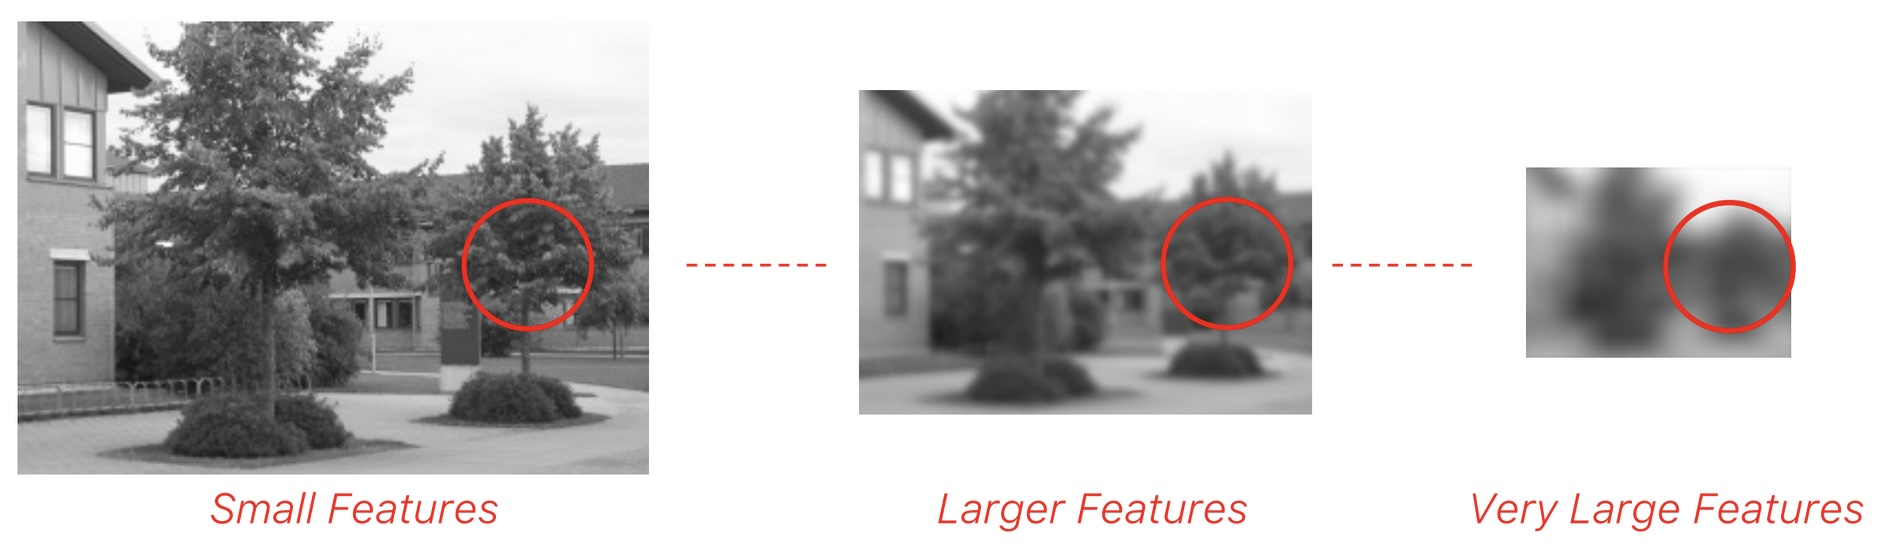
\includegraphics[width=0.9\linewidth]{./img/scale_space.jpg}
  \caption{A scale-space pyramid: the image is progressively blurred (increasing $\sigma$) and often downsampled to create different octaves. Within an octave, $\sigma$ increases.}
  \label{fig:scale_space}
\end{figure}

\paragraph{Feature Detection and Characteristic Scale Selection}
While the scale-space represents the image across various scales, criteria are needed to detect salient features and determine their "characteristic scale" – the scale at which a feature is most prominent.
Derivatives (used in many feature detectors) tend to weaken as the smoothing scale $\sigma$ increases. To counteract this and enable fair comparison of feature responses across scales, Lindeberg proposed \textbf{scale normalization}: multiplying derivatives by an appropriate power of $\sigma$.

\paragraph{Scale-Normalized Laplacian of Gaussian (LoG)}
For blob detection (regions that are brighter or darker than their surroundings), the scale-normalized Laplacian of Gaussian (LoG) can be used. The LoG operator combines Gaussian smoothing with the Laplacian operator ($\nabla^2$). Its scale-normalized form is:
\[ F_{norm}(x,y,\sigma) = \sigma^2 \nabla^2 L(x,y,\sigma) = \sigma^2 (\nabla^2 G(x,y,\sigma) * I(x,y)) \]
The $\sigma^2$ factor compensates for the natural decay of the Laplacian response with increasing $\sigma$, preventing a bias towards detecting only small-scale features. Extrema (maxima or minima) of $F_{norm}(x,y,\sigma)$ in both space $(x,y)$ and scale $(\sigma)$ indicate the centers and characteristic scales of blob-like features.

\begin{figure}[htbp]
  \centering
  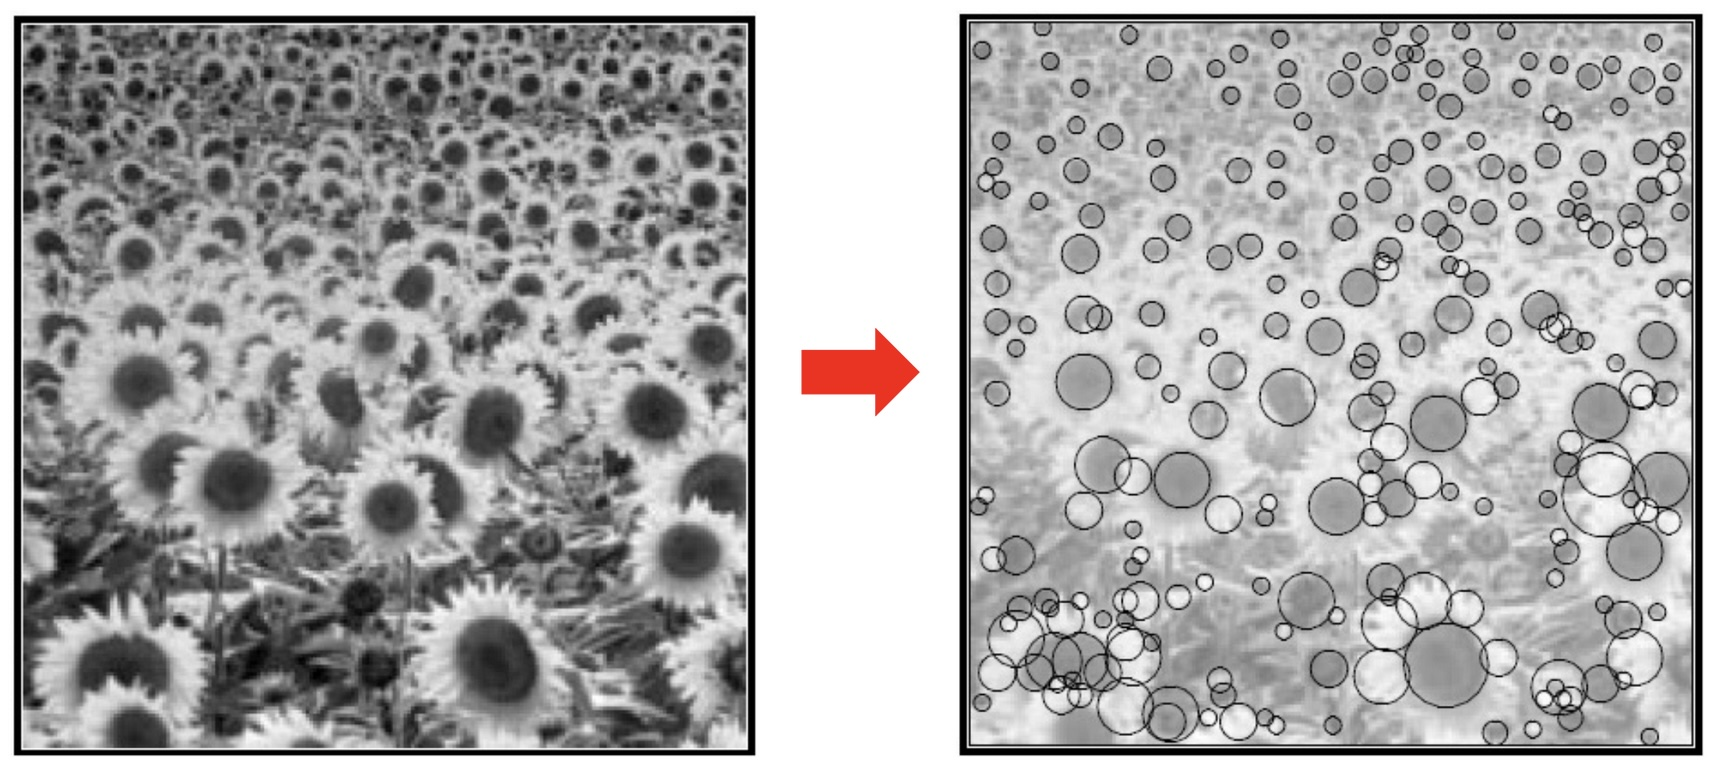
\includegraphics[width=0.7\linewidth]{./img/sunflower_blobs.jpg}
  \caption{Blobs detected by a LoG-like filter at their characteristic scales.}
  \label{fig:sunflower_blobs}
\end{figure}

\paragraph{Difference of Gaussian (DoG)}
Computing the LoG and its extrema across a finely sampled scale-space can be computationally intensive. Lowe, in the SIFT (Scale Invariant Feature Transform) framework, proposed using the Difference of Gaussians (DoG) function as an efficient approximation:
\[ DoG(x,y,\sigma) = (G(x,y,k\sigma) - G(x,y,\sigma)) * I(x,y) = L(x,y,k\sigma) - L(x,y,\sigma) \]
where $k$ is a constant factor between the scales of two nearby smoothed images. The DoG function approximates the scale-normalized LoG because the difference of two Gaussian kernels, $G(x,y,k\sigma) - G(x,y,\sigma)$, approximates $(k-1)\sigma^2 \nabla^2 G(x,y,\sigma)$. Thus, local extrema of the DoG function in space and scale serve as candidate keypoints. The DoG operator, being composed of isotropic Gaussian kernels, is inherently rotation invariant.

\begin{figure}[htbp]
  \centering
  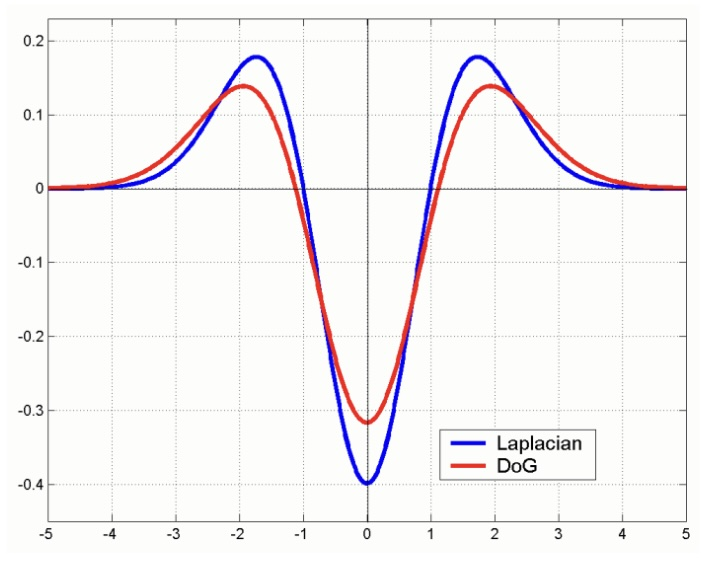
\includegraphics[width=0.5\linewidth]{./img/dog.jpg}
  \caption{The Difference of Gaussians (DoG) kernel (bottom) as an approximation of the Laplacian of Gaussian (LoG) kernel (top, scaled). The DoG is computationally cheaper.}
  \label{fig:dog}
\end{figure}

In practice, the scale-space is often organized into "octaves," where each octave corresponds to a doubling of $\sigma$. Within an octave, several DoG images are computed by subtracting adjacent Gaussian-smoothed images.

\begin{figure}[htbp]
  \centering
  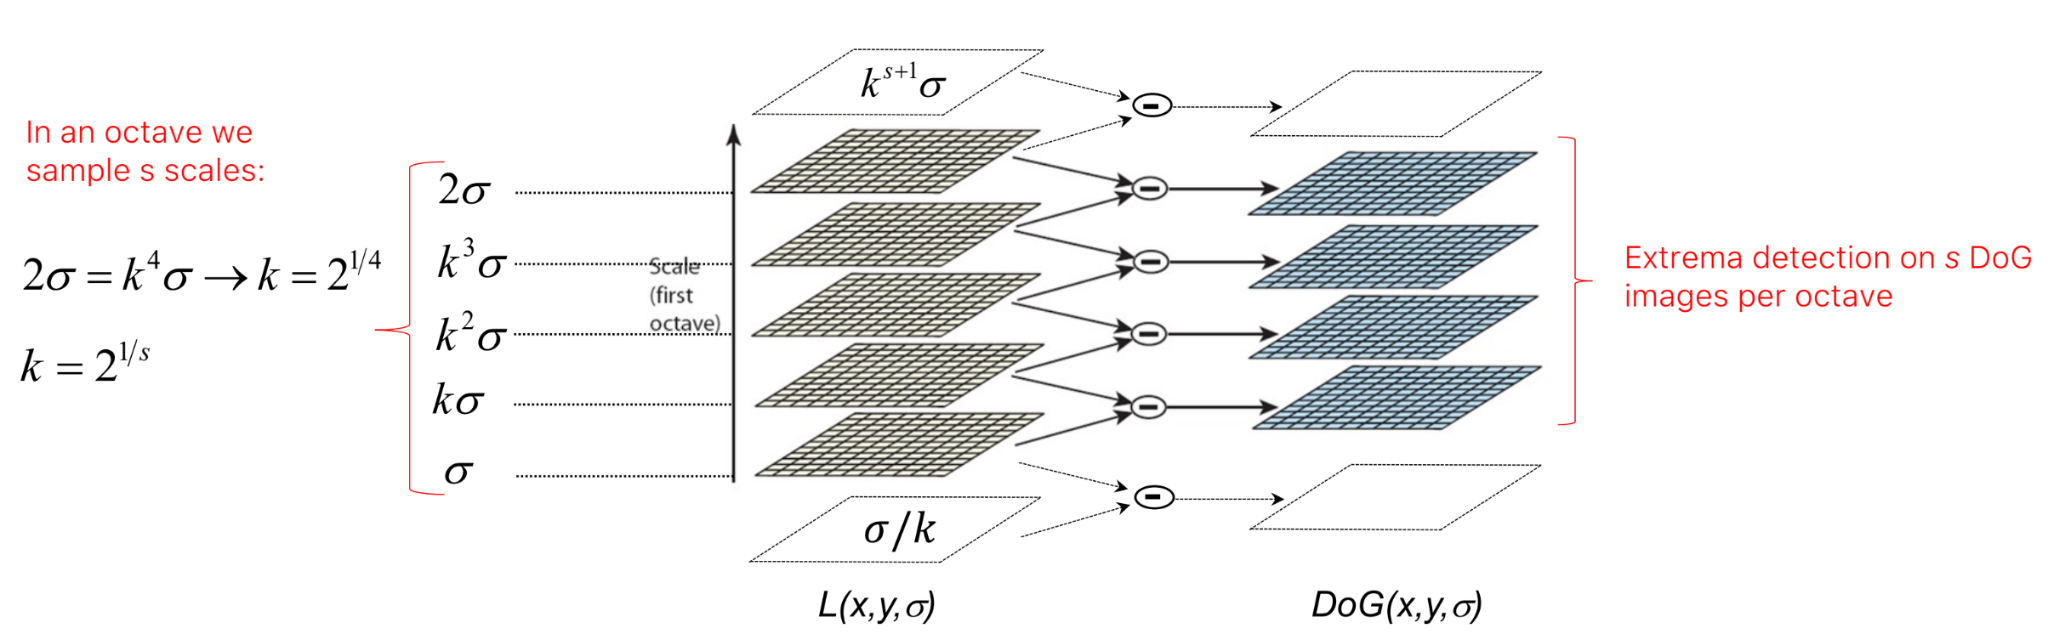
\includegraphics[width=0.9\linewidth]{./img/dog_1.png}
  \caption{Generation of Difference of Gaussian (DoG) images. An image is repeatedly smoothed (intra-octave scales), and differences between adjacent smoothed images form the DoG layers. The image may also be downsampled to start a new octave.}
  \label{fig:dog_1}
\end{figure}

\paragraph{Extrema Detection and Refinement}
A point $(x,y,\sigma)$ is detected as a keypoint candidate if its DoG value is a local extremum (maximum or minimum) compared to its 26 neighbors in the $3 \times 3 \times 3$ region of DoG images (8 neighbors at the same scale, and 9 neighbors each at the scales above and below).
Lowe's original SIFT paper suggests specific parameters, such as an initial $\sigma_0 = 1.6$, $s=3$ images to be detected per octave (requiring $s+3$ smoothed images), and often starting by up-sampling the input image by a factor of 2.

Candidate keypoints are then refined:
\begin{itemize}
    \item \textbf{Accurate localization}: Sub-pixel and sub-scale localization is performed by fitting a 3D quadratic function to the DoG values around the candidate.
    \item \textbf{Thresholding low-contrast responses}: Keypoints with low DoG magnitudes (low contrast) are discarded as they are sensitive to noise.
    \item \textbf{Eliminating edge responses}: DoG produces strong responses along edges. These are unstable for localization and are removed using a method similar to the Harris corner detector, by checking the ratio of principal curvatures (eigenvalues of the Hessian matrix of the DoG function).
\end{itemize}

\begin{figure}[htbp]
  \centering
  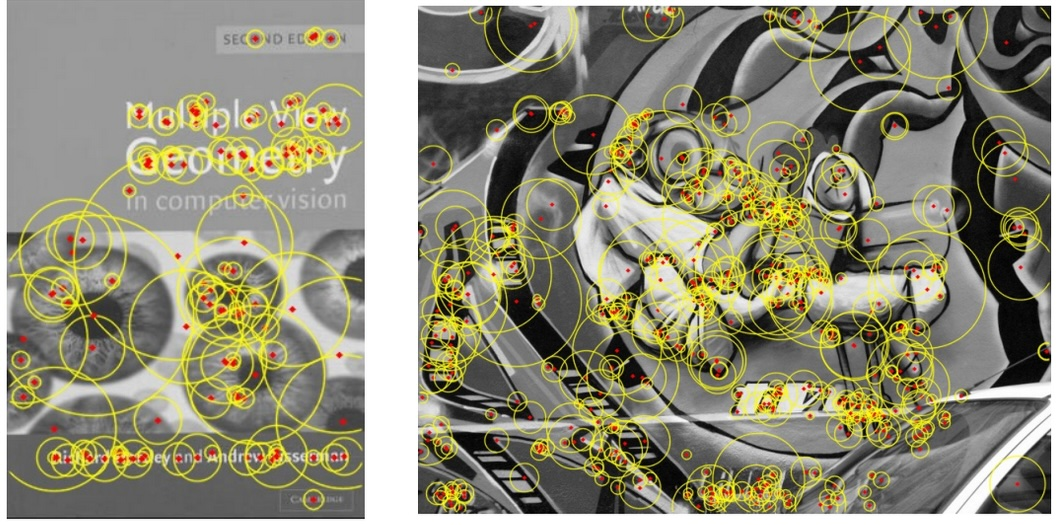
\includegraphics[width=0.7\linewidth]{./img/dog_keypoints.jpg}
  \caption{Keypoints detected using DoG. The size of each circle is proportional to the characteristic scale ($\sigma$) of the detected feature.}
  \label{fig:dog_keypoints}
\end{figure}

\subsubsection{Scale and Rotation Invariant Description}
Once stable keypoints are detected along with their characteristic scales, descriptors are computed to capture the local image information. These descriptors must also be invariant to scale and rotation.

\begin{itemize}
  \item \textbf{Scale invariance} is achieved by computing the descriptor on the image patch corresponding to the keypoint's characteristic scale (i.e., from the Gaussian-smoothed image $L(x,y,\sigma_i)$ where $\sigma_i$ is the scale of detection). The size of the descriptor's support region is scaled proportionally to $\sigma_i$.
  \item \textbf{Rotation invariance} is achieved by assigning a \textit{canonical orientation} to each keypoint. The descriptor is then computed relative to this orientation.
\end{itemize}

Lowe proposed computing the canonical orientation(s) as follows:
For each keypoint, consider its corresponding Gaussian-smoothed image $L(x,y,\sigma_i)$.
\begin{enumerate}
  \item Compute gradient magnitude $m(x,y)$ and orientation $\theta(x,y)$ for pixels in a neighborhood around the keypoint in $L(x,y,\sigma_i)$:
    \begin{align*}
        m(x,y) &= \sqrt{(L(x+1,y)-L(x-1,y))^2 + (L(x,y+1) - L(x,y-1))^2} \\
        \theta(x,y) &= \arctan^2(L(x,y+1)-L(x,y-1), L(x+1,y)-L(x-1,y))
    \end{align*}
  \item Create an orientation histogram from these gradients. The histogram typically has 36 bins (covering $360^\circ$ in $10^\circ$ increments). Each sample added to the histogram is weighted by its gradient magnitude and by a Gaussian window centered at the keypoint (with $\sigma$ proportional to the keypoint's scale).
  \item The highest peak in the orientation histogram defines the dominant orientation for the keypoint. Any other local peaks within 80\% of the highest peak also define additional orientations. This means a single keypoint location/scale can result in multiple feature descriptors if it has multiple prominent orientations (occurring for about 15\% of keypoints, often at symmetric locations).
\end{enumerate}

\begin{figure}[htbp]
  \centering
  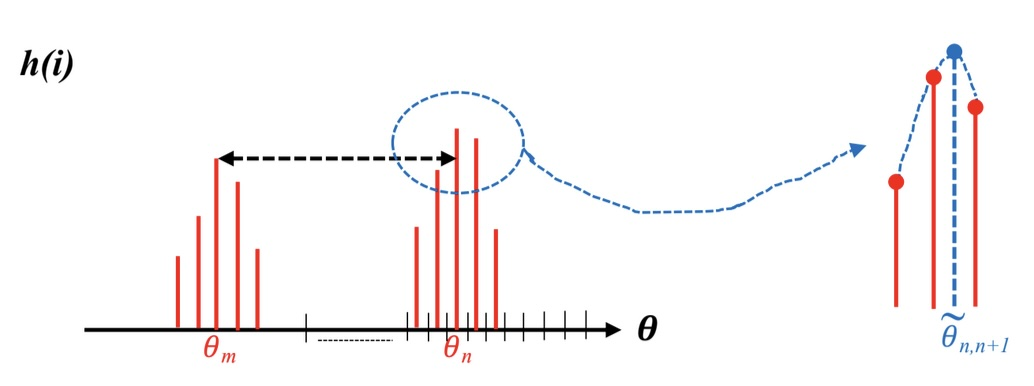
\includegraphics[width=0.7\linewidth]{./img/ambiguous_keypoint.jpg}
  \caption{An example of a keypoint with ambiguous orientation, potentially leading to two dominant directions in the orientation histogram.}
  \label{fig:ambiguous_keypoints}
\end{figure}

\subsubsection{The SIFT Descriptor}
The SIFT (Scale Invariant Feature Transform) descriptor is computed for each keypoint (and each of its canonical orientations) as follows:
\begin{enumerate}
  \item A $16 \times 16$ pixel neighborhood around the keypoint is selected from the Gaussian-smoothed image $L(x,y,\sigma_i)$ corresponding to the keypoint's scale. This patch is rotated to align with the keypoint's canonical orientation.
  \item This $16 \times 16$ patch is divided into a $4 \times 4$ grid of $4 \times 4$ pixel subregions.
  \item For each $4 \times 4$ subregion, an 8-bin gradient orientation histogram is computed. Gradients are relative to the keypoint's canonical orientation.
  \item Each pixel in a subregion contributes to its orientation histogram, weighted by its gradient magnitude and a Gaussian window (with $\sigma$ equal to half the width of the $16 \times 16$ grid) centered on the keypoint. This down-weights gradients far from the keypoint center.
\end{enumerate}
The resulting descriptor is a vector of $4 \times 4 \times 8 = 128$ values. This vector is then normalized to unit length to achieve robustness to affine illumination changes (brightness and contrast).

\begin{figure}[htbp]
  \centering
  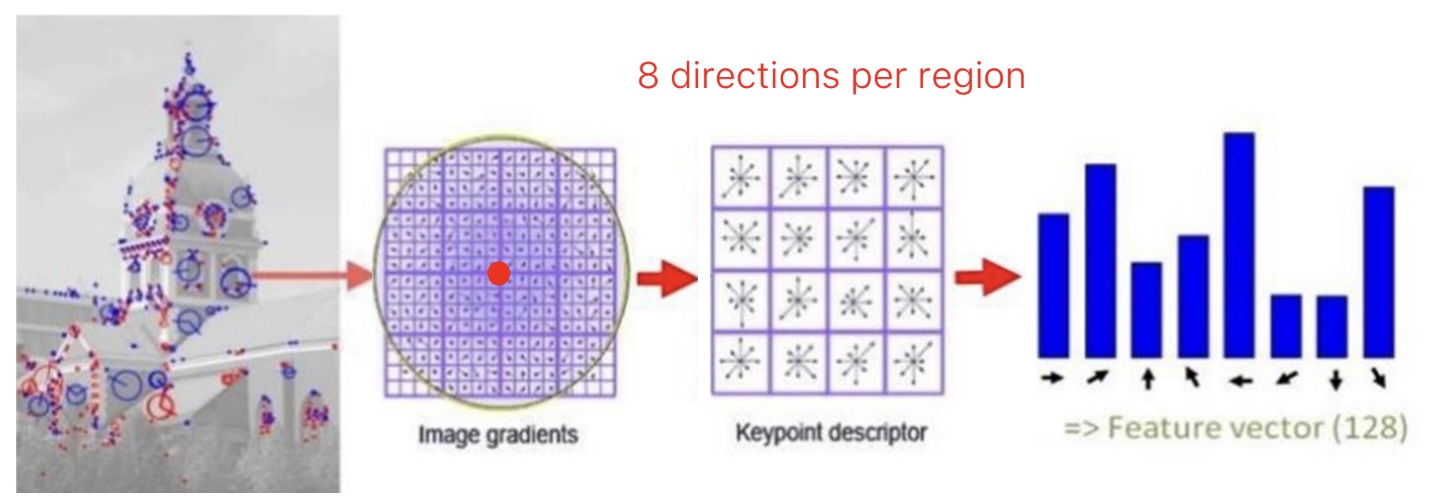
\includegraphics[width=0.8\linewidth]{./img/sift_descriptor.jpg}
  \caption{SIFT descriptor computation: A $16 \times 16$ window (rotated to canonical orientation) is divided into $4 \times 4$ subregions. Each subregion contributes an 8-bin orientation histogram. Total descriptor length is $4 \times 4 \times 8 = 128$.}
  \label{fig:sift_descriptor}
\end{figure}

\paragraph{Matching Process}
To find corresponding keypoints between two images (a query image $Q$ and a reference image $R$), their SIFT descriptors are compared. This is a Nearest Neighbor (NN) search problem in the 128-dimensional descriptor space.
For each SIFT feature $f_Q$ in the query image, its nearest neighbor $f_{R1}$ (most similar descriptor) in the reference image is found using Euclidean distance.

However, the nearest neighbor might not be a correct match (e.g., if $f_Q$ has no true correspondent in $R$). To improve reliability, Lowe proposed a ratio test:
Compare the distance to the nearest neighbor ($d_1$) with the distance to the second nearest neighbor ($d_2$). If $d_1 / d_2 < T_{ratio}$ (e.g., $T_{ratio} = 0.8$), the match is accepted. Otherwise, it is rejected as ambiguous. This threshold effectively rejects many false matches while retaining most correct ones.

Exhaustive NN search is computationally expensive ($O(N M D)$ where $N, M$ are numbers of features and $D$ is descriptor dimensionality). Approximate nearest neighbor algorithms, such as those based on k-d trees (e.g., Best Bin First search), are used to speed up the matching process significantly for large databases of features.

\begin{figure}[htbp]
  \centering
  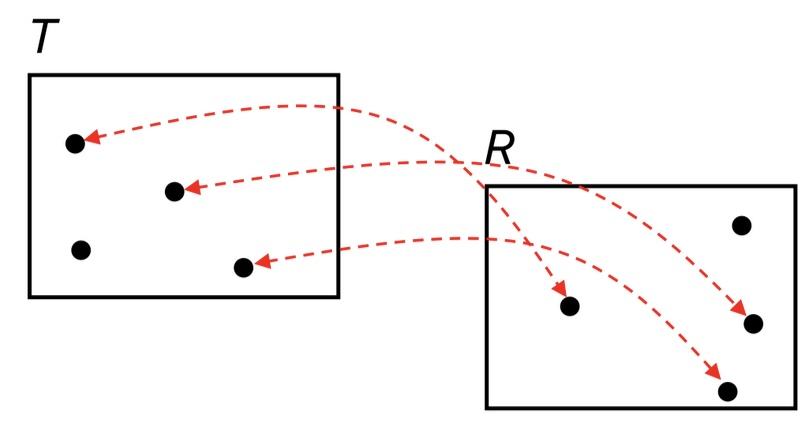
\includegraphics[width=0.5\linewidth]{./img/matching_sift.jpg}
  \caption{Matching SIFT features between two images. Lines connect corresponding keypoints.}
  \label{fig:matching_sift}
\end{figure}

% ==============================================================================

% \subsection{Camera Calibration}

% Camera Calibration is important for taking quantitative measurements from images.
% In the \textbf{perspective projection} model, given a point in the 3D space $M = [x,y,z]^T$, with coordinates given in the Camera Reference Frame (CRF).
% Its projection onto the image plane I is denoted as $m=[u,v]^T$.

% \begin{figure}[htbp]
%   \centering
%   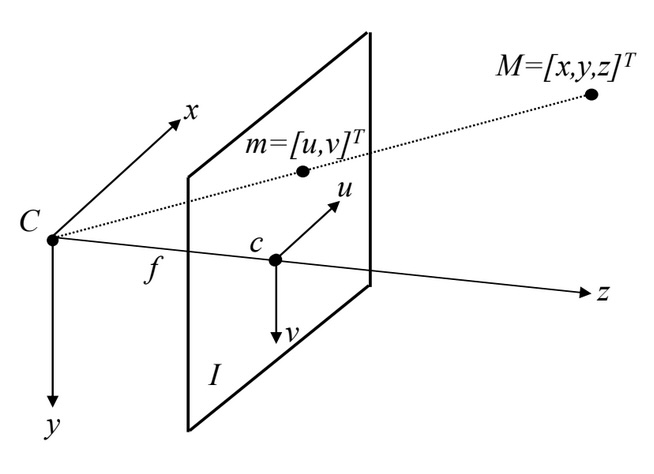
\includegraphics[width=0.5\linewidth]{./img/camera_calibration.jpg}
%   \caption{Perspective Projection Model (PPM)}
%   \label{fig:camera calibration}
% \end{figure}

% \subsubsection{Projective Space}

% The \textbf{Physical Space} is a 3D Euclidean Space ($\mathbb{R}^3$) whose points can be represented as 3D vectors in a given reference frame.
% In this space parallel lines do not intersect.
% Points at infinity cannot be represented in this vector space.

% The \textbf{Projective Space} is a mathematical engine to handle the geometry of image formations.
% In the Projective space we append one more coordinate to the Euclidean triplets.
% A point is represented by an equivalence class of quadruples, wherein equivalent quadruples differ just by a multiplicative factor.
% This is called the \textbf{homogeneous coordinates} representation of the 3D point having Euclidean coordinates $(x,y,z)$.
% The space associated with the homogeneous coordinate's representation is called Projective Space, denoted as $P^3$

% \vspace{0.6em}
% We are interested in Projective Spaces because Perspective Projection is \textbf{more conveniently} dealt with using projective coordinates.
% \vspace{0.6em}

% The point at infinity is a point in the space, the vanishing point is a point into the image plane.
% Points at infinity of the 3D lines are the points of the 3D Projective Space \textbf{having the fourth coordinate equal to 0}.

% To map such points into the Euclidean Space we would divide by the fourth coordinate (which is 0) which is not a valid representation in the Euclidean Space.

% The point $(0,0,0,0)$ it's not the origin, but an undefined point. The origin is represented in homogeneous coordinates as $(0,0,0,k)$, with $k\neq 0$.

% Given a 3D point $\tilde{M} = [x,y,z]^T$ (with coordinates expressed in the Camera Reference Frame) and its 2D projection onto the image plane $\tilde{m} = [u,v]^T$.

% In homogeneous coordinates the perspective projection becomes a linear transformation.

% $$
% \begin{bmatrix}
% u \\ v \\ 1
% \end{bmatrix} =
% \begin{bmatrix}
% f & 0 & 0 & 0 \\
% 0 & f & 0 & 0 \\
% 0 & 0 & 1 & 0 
% \end{bmatrix}
% \begin{bmatrix}
% x \\ y \\ z \\ 1
% \end{bmatrix}
% $$

% Which in matrix notation is $\tilde{m} \approx \tilde{P}\tilde{M}$, where $\approx$ means "equal up to an arbitrary scale factor".
% \vspace{1em}
% $\tilde{P}$ represents the geometric camera model, and is known as \textbf{Perspective Projection Matrix (PPM)}.

% \vspace{1em}

% The operation carried out by the PPM is that of scaling lateral coordinates according to the distance from the camera $(z)$.
% The actual focal length just introduces an additional scaling factor of projected coordinates.

% \subsubsection{A more comprehensive camera model}

% To create a more realistic camera model we need to consider three additional issues:
% \begin{enumerate}
%   \item Image coordinates are usually expresed in an image reference frame with the origin in the top left corner.
%   \item Images are a grid of pixels, not a continuous plane (pixelization).  The digitization can be accounted for by including into the projection equations the pixel size $\Delta u$ and $\Delta v$ along the two axes (typically they have the same value).
%   \item We do not normally know or want to project back the coordinate of a 3D point in the Camera Reference Frame, but in some generic World Reference Frame, that we place where it's most comfortable for us.
% \end{enumerate}

% \paragraph{Intrinsic Parameter Matrix}

% The matrix $A$, models the intrinsic characteristics (Intrinsic Parameters) of the image sensing device (focal length, pixel dimension...) and is called \textbf{Intrinstic Parameter Matrix}
% The smallest number of intrinsic parameters is thus 4 ($f_u, f_v$ and the coordinates of the piercing point $c(u_0, v_0)$).
% They represent the camera geometry, which is independent of its position in the world.

% Now the Perspective Projection Matrix can be written as:
% $$
% \tilde{P} = 
% \begin{bmatrix}
%   fk_u & 0 & u_0 & 0 \\
%   0 & fk_v & v_0 & 0 \\
%   0 & 0 & 1 & 0 
% \end{bmatrix}
% =
% \begin{bmatrix}
%   fk_u & 0 & u_0 \\
%   0 & fk_v & v_0 \\
%   0 & 0 & 1 
% \end{bmatrix}
% \begin{bmatrix}
%   1 & 0 & 0 & 0 \\
%   0 & 1 & 0 & 0 \\
%   0 & 0 & 1 & 0 
% \end{bmatrix}
% = A[I|0]
% $$

% We can now see that if we have $[a,b,c,0]$, which are the coordinates of a point in the WRF. By using the Perspective Projection matrix we can do this calculation:

% $$
% \tilde{m}_{\infty} =
% P_{int}
% \begin{bmatrix}
% a \\ b \\ c \\ 0
% \end{bmatrix}
% =
% \begin{bmatrix}
%   fk_u & 0 & u_0 & 0 \\
%   0 & fk_v & v_0 & 0 \\
%   0 & 0 & 1 & 0 
% \end{bmatrix}
% \begin{bmatrix}
% a \\ b \\ c \\ 0
% \end{bmatrix}
% =
% \begin{bmatrix}
% f_u a + c u_0 \\
% f_v b + c v_0 \\
% c
% \end{bmatrix}
% $$

% The final vector can be divided by $c$ (the third component) and we get the coordinates of the point at infinity in an image: $m_{\infty} = \begin{bmatrix} f_u \frac{a}{c} + u_0 \\ f_v \frac{b}{c} + v_0\end{bmatrix}$.

% This handles all the cases except $c = 0$, which is the case of a line parallel to the camera sensor.

% \paragraph{Rigid motion between CRF and WRF}
% We need to apply a roto-translation to relate the World Reference Frame to the Camera Reference Frame.
% The relation between the coordinates of a point in the two reference frames is:

% $$
% W =
% \begin{bmatrix}
% X \\ Y \\ Z \\ 1
% \end{bmatrix}
% \,,
% M=
% \begin{bmatrix}
% x\\ y\\ z\\1
% \end{bmatrix}
% \Rightarrow
% M=
% \begin{bmatrix}
% R & T \\
% 0 & 1
% \end{bmatrix}
% W = GW
% $$

% To map a 3D point expressed in the Camera Reference Frame: $k\tilde{m} = A[I|0]\tilde{M}$

% The general from of the Perspective Projection Matrix can be expressed as follows:
% $\tilde{P} = A[I|0]G$ or also $\tilde{P}=A[R|T]$.

% \paragraph{Extrinsic Parameters}

% $G$ is called \textbf{Extrinsic Parameter Matrix} and it encodes the position and orientation of the camera with respect to the World Reference Frame.
% The rotation matrix has only 3 independent parameters, which correspond to the rotation angles around the axis of the reference frame.
% $T$ has 3 independent parameters.
% The total number of \textbf{extrinsic parameters} is 6 (3 translation, 3 rotation).
% $A$ has 4 independent parameters.
% The general form of the Perspective Projection Matrix can be thought of as encoding:
% \begin{itemize}
%   \item the position of the camera with respect to the world into $G$.
%   \item the actual characteristics of the sensing device into $A$.
% \end{itemize}

% ==============================================================================

\subsection{Camera Calibration}

Camera calibration is the process of determining the parameters of a camera model that describes how a 3D scene is projected onto a 2D image. This is crucial for extracting quantitative measurements from images, such as object sizes or distances. We primarily focus on the \textbf{perspective projection} model.

\begin{figure}[htbp]
  \centering
  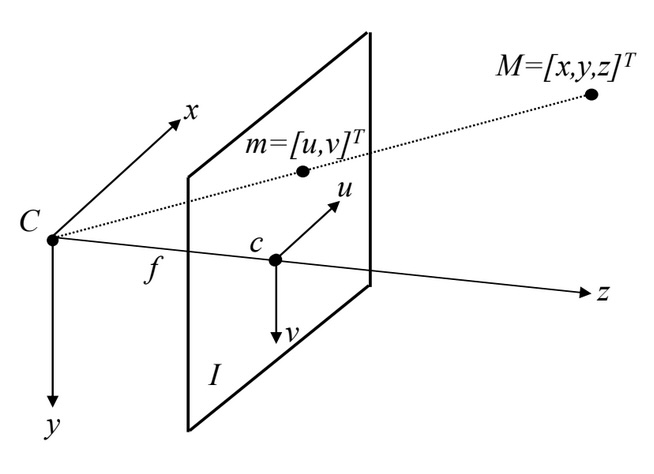
\includegraphics[width=0.5\linewidth]{./img/camera_calibration.jpg}
  \caption{Perspective Projection Model (PPM). A 3D point $M$ in the Camera Reference Frame (CRF) projects to a 2D point $m$ on the image plane $I$.}
\end{figure}

\subsubsection{From Physical Space to Projective Space}

The world we perceive is often modeled as a 3D \textbf{Euclidean Space} ($\mathbb{R}^3$). Points are represented by 3D vectors $[x, y, z]^T$ in a chosen reference frame. However, Euclidean geometry struggles with concepts like points at infinity and the projective nature of image formation (e.g., parallel lines appearing to converge).

To handle the geometry of perspective projection more elegantly, we use \textbf{Projective Space} ($P^3$).
\begin{itemize}
    \item \textbf{Homogeneous Coordinates:} A point with Euclidean coordinates $(x, y, z)$ is represented in homogeneous coordinates by an equivalence class of 4D vectors $[\lambda x, \lambda y, \lambda z, \lambda]^T$ for any non-zero scalar $\lambda$. A common choice is to set $\lambda=1$, giving $[x, y, z, 1]^T$.
    \item \textbf{Mapping Back:} To convert from homogeneous coordinates $[X, Y, Z, W]^T$ (where $W \neq 0$) back to Euclidean coordinates, we divide by the fourth component: $[X/W, Y/W, Z/W]^T$.
    \item \textbf{Points at Infinity:} Points at infinity correspond to directions in 3D space. In homogeneous coordinates, they are represented by vectors of the form $[X, Y, Z, 0]^T$, where $[X, Y, Z]^T$ defines the direction. These points cannot be mapped back to the finite Euclidean space.
    \item \textbf{The Origin:} The origin of the Euclidean space $(0,0,0)$ is represented by $[0, 0, 0, k]^T$ with $k \neq 0$ in homogeneous coordinates. The vector $[0, 0, 0, 0]^T$ is undefined in projective space.
\end{itemize}
The main advantage of using homogeneous coordinates is that the non-linear perspective projection equations become \textbf{linear transformations} represented by matrix multiplication.

\subsubsection{Basic Perspective Projection Matrix (Pinhole Camera)}

Let $M = [x, y, z]^T$ be a 3D point expressed in the \textbf{Camera Reference Frame (CRF)}, with the origin at the camera's optical center and the z-axis along the optical axis. Let its projection onto the image plane be $m = [u, v]^T$. Assuming the image plane is at $z=f$ (where $f$ is the focal length), the basic perspective projection is:
$u = f \frac{x}{z}$ and $v = f \frac{y}{z}$.

Using homogeneous coordinates, we represent the 3D point as $\tilde{M}_{CRF} = [x, y, z, 1]^T$ and the projected 2D point as $\tilde{m} = [u', v', w']^T$, where the final image coordinates are $u = u'/w'$ and $v = v'/w'$. The projection can be written as a linear mapping:

\[
w' % Scaling factor, which turns out to be z
\begin{bmatrix}
u \\ v \\ 1
\end{bmatrix}
=
\begin{bmatrix}
f & 0 & 0 & 0 \\
0 & f & 0 & 0 \\
0 & 0 & 1 & 0
\end{bmatrix}
\begin{bmatrix}
x \\ y \\ z \\ 1
\end{bmatrix}
\]
This can be written compactly as $\tilde{m} \propto P_0 \tilde{M}_{CRF}$, where $\propto$ denotes equality up to a non-zero scale factor, and $P_0$ is the basic $3 \times 4$ perspective projection matrix for a pinhole camera centered at the origin, looking along the z-axis. The scale factor here is $w'=z$.

\subsubsection{A More Comprehensive Camera Model}

The basic model is often insufficient. We need to account for:
\begin{enumerate}
  \item \textbf{Image Coordinate System:} Image coordinates $(u, v)$ are typically measured in pixels, with the origin often at the top-left corner, not the principal point (where the optical axis pierces the image plane).
  \item \textbf{Pixel Shape:} Pixels might not be square. We need parameters for pixel size/density $(\Delta u, \Delta v)$ or equivalently, focal lengths measured in pixels ($f_u = f/\Delta u$, $f_v = f/\Delta v$).
  \item \textbf{World Reference Frame (WRF):} 3D points are usually defined in a convenient WRF, not the CRF. We need to relate the WRF to the CRF.
\end{enumerate}

These factors lead to a more complex projection matrix $\tilde{P}$, which can be decomposed into intrinsic and extrinsic parameters.

\paragraph{Intrinsic Parameter Matrix (A)}
This $3 \times 3$ matrix maps projected points from the camera's normalized image plane (where $z=1$) to pixel coordinates. It encodes the camera's internal geometry:
\begin{itemize}
    \item $f_u, f_v$: Focal lengths expressed in units of horizontal and vertical pixel dimensions.
    \item $(u_0, v_0)$: Coordinates of the principal point (the image center) in pixels. Sometimes denoted $(c_x, c_y)$.
\end{itemize}
Assuming zero skew, the intrinsic matrix is:
\[
A =
\begin{bmatrix}
  f_u & 0 & u_0 \\
  0 & f_v & v_0 \\
  0 & 0 & 1
\end{bmatrix}
\]
These \textbf{intrinsic parameters} (at least 4: $f_u, f_v, u_0, v_0$) are specific to the camera and lens, independent of the camera's position or orientation in the world.

The projection from the CRF using only intrinsic parameters can be written by combining $A$ with a standard projection into the normalized image plane:
\[
\tilde{P}_{int} = A [I | \mathbf{0}] =
\begin{bmatrix}
  f_u & 0 & u_0 & 0 \\
  0 & f_v & v_0 & 0 \\
  0 & 0 & 1 & 0
\end{bmatrix}
\]
This matrix $\tilde{P}_{int}$ maps a 3D point in homogeneous coordinates \emph{relative to the CRF} to its 2D homogeneous pixel coordinates.

\paragraph{Vanishing Points Example}
Consider a point at infinity $[a, b, c, 0]^T$ representing a direction relative to the CRF. Its projection using $\tilde{P}_{int}$ is:
\[
\tilde{m}_{\infty} \propto \tilde{P}_{int}
\begin{bmatrix} a \\ b \\ c \\ 0 \end{bmatrix}
=
\begin{bmatrix}
  f_u a + u_0 c \\
  f_v b + v_0 c \\
  c
\end{bmatrix}
\]
Assuming $c \neq 0$ (the direction is not parallel to the image plane), we can convert to Euclidean pixel coordinates by dividing by the third component:
\[
m_{\infty} = \begin{bmatrix} f_u \frac{a}{c} + u_0 \\ f_v \frac{b}{c} + v_0 \end{bmatrix}
\]
This projected point $m_{\infty}$ is a \textbf{vanishing point} in the image – the point where parallel lines in 3D space with direction $[a, b, c]^T$ appear to converge. If $c=0$, the direction is parallel to the image plane, and the point projects to infinity in the image plane coordinates (no finite vanishing point).


\paragraph{Extrinsic Parameter Matrix (G)}
To use points defined in a World Reference Frame (WRF), we need to describe the camera's pose (position and orientation) relative to the WRF. This is done using a rigid body transformation:
\begin{itemize}
    \item $R$: A $3 \times 3$ rotation matrix describing the orientation of the CRF relative to the WRF.
    \item $T$: A $3 \times 1$ translation vector describing the position of the CRF origin relative to the WRF origin (expressed in WRF coordinates). Or sometimes, the position of the WRF origin relative to the CRF origin (expressed in CRF coordinates) - convention matters! Let's assume $T$ specifies the CRF origin in WRF for the $G$ matrix below which transforms points *from* WRF *to* CRF.
\end{itemize}
The transformation from WRF coordinates $\tilde{M}_W = [X, Y, Z, 1]^T$ to CRF coordinates $\tilde{M}_{CRF} = [x, y, z, 1]^T$ is given by:
\[
\tilde{M}_{CRF} = G \tilde{M}_W
\]
where $G$ is the $4 \times 4$ \textbf{Extrinsic Parameter Matrix}. A common form relates WRF coordinates to CRF coordinates:
\[
G = \begin{bmatrix} R & T \\ \mathbf{0}^T & 1 \end{bmatrix}
\]
Here, $R$ rotates the WRF axes to align with the CRF axes, and $T$ translates the origin. This transformation has \textbf{6 extrinsic parameters}: 3 for rotation (e.g., Euler angles, axis-angle) and 3 for translation.

The transformation from WRF to CRF coordinates (non-homogeneous) is $M_{crf} = R M_w + T'$, where $T'$ is the translation vector. In homogeneous coordinates, this is often expressed using a $4\times4$ matrix that incorporates the inverse transformation or directly within the projection matrix.

\subsubsection{The Complete Perspective Projection Matrix (\~{P})}

Combining the intrinsic and extrinsic parameters, the full projection from a 3D point $\tilde{M}_W$ in WRF homogeneous coordinates to a 2D point $\tilde{m}$ in image homogeneous pixel coordinates is:
\[
\tilde{m} \propto A [R | T] \tilde{M}_W
\]
Here, the $3 \times 4$ matrix $\tilde{P} = A[R|T]$ is the complete \textbf{Perspective Projection Matrix (PPM)}.
\begin{itemize}
    \item $R$ is the $3 \times 3$ rotation matrix specifying the camera's orientation.
    \item $T$ is the $3 \times 1$ translation vector specifying the camera's position (specifically, $T = -RC_W$, where $C_W$ is the position of the camera center in world coordinates).
\end{itemize}
The matrix $[R|T]$ effectively transforms the point from WRF coordinates directly into the CRF, ready for projection and intrinsic transformation by $A$.

The PPM $\tilde{P}$ encodes all the geometric information of the camera setup:
\begin{itemize}
    \item Intrinsic parameters ($A$): Camera's internal geometry (focal length, principal point, pixel properties). (4+ parameters)
    \item Extrinsic parameters ($R, T$): Camera's pose (position and orientation) in the world. (6 parameters)
\end{itemize}
Camera calibration aims to find the numerical values for the parameters in $A$ and, often simultaneously or subsequently, the extrinsic parameters $R$ and $T$ relative to a known calibration target.

\subsubsection{P as a Homography}
We just need the relation between the camera and the plane, then we can measure everything on that plane.

If the camera is imaging a planar scene, we can assume the z-axis of the World Reference Frame to be perpendicular to the plane such that all 3D points will have their z-coordinate equal to 0.
The Perspective Projection Matrix then becomes a simpler transformation defined by a $3x3$ matrix.
$$k\tilde{m} = \tilde{P}\tilde{w}
\begin{bmatrix}
  p_{1,1} & p_{1,2} & \cancel{p_{1,3}} & p_{1,4} \\
  p_{2,1} & p_{2,2} & \cancel{p_{2,3}} & p_{2,4} \\
  p_{3,1} & p_{3,2} & \cancel{p_{3,3}} & p_{3,4} 
\end{bmatrix}
\begin{bmatrix}
x \\ y \\ 0 \\ 1
\end{bmatrix}
=
\begin{bmatrix}
  p_{1,1} & p_{1,2} & p_{1,4} \\
  p_{2,1} & p_{2,2} & p_{2,4} \\
  p_{3,1} & p_{3,2} & p_{3,4} 
\end{bmatrix}
\begin{bmatrix}
x \\ y \\ 1
\end{bmatrix}
= H\tilde{M}
$$

Such a transformation, denoted here as H, is known as \textbf{homography} and represents a general linear transformation between projective planes.
A homography is then a projective transformation between two planes or a mapping between two planar projection of an image.

\begin{figure}[htbp]
  \centering
  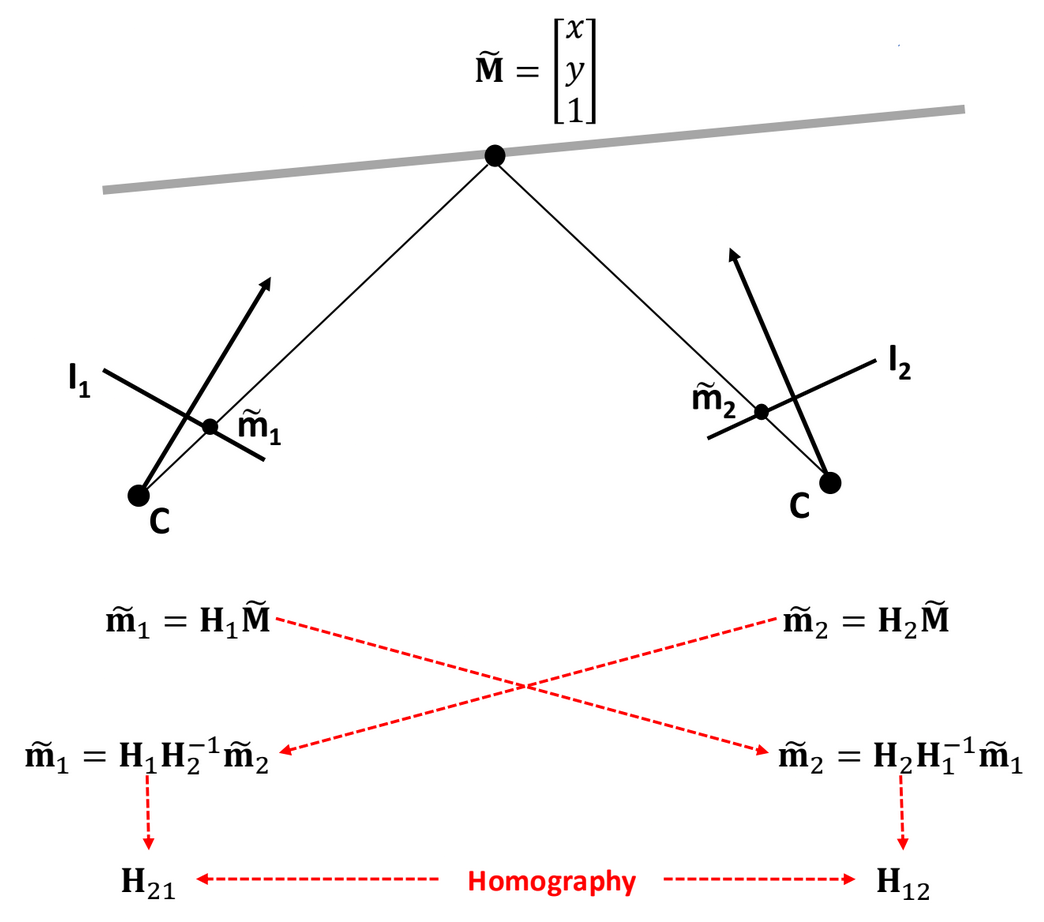
\includegraphics[width=0.6\linewidth]{./img/homography.jpg}
  \caption{Any two images of a planar scene are related by a homography}
  \label{fig:homography}
\end{figure}

\begin{figure}[htbp]
  \centering
  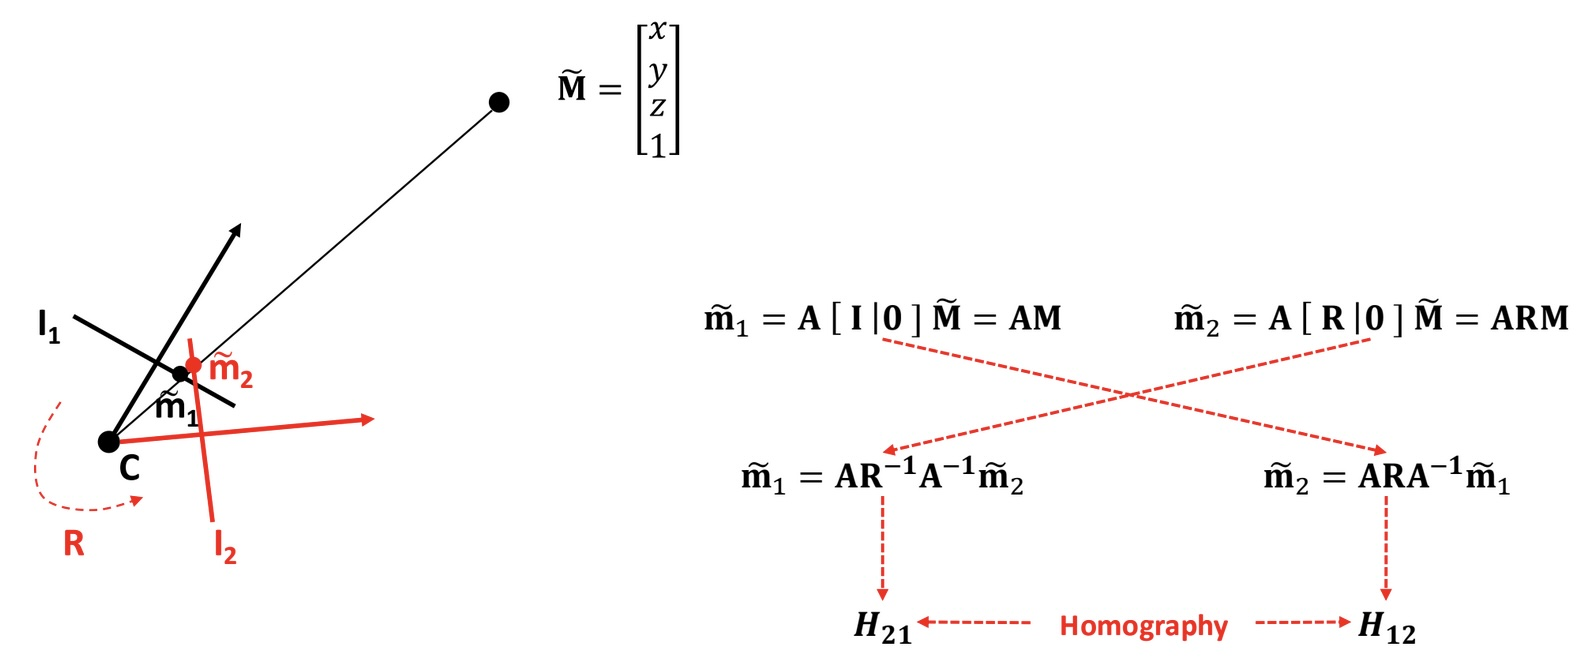
\includegraphics[width=0.8\linewidth]{./img/rotating_homography.jpg}
  \caption{Any two images taken by a camera rotating about the optical center are related by a homography}
  \label{fig:rotating_homography}
\end{figure}

\begin{figure}[htbp]
  \centering
  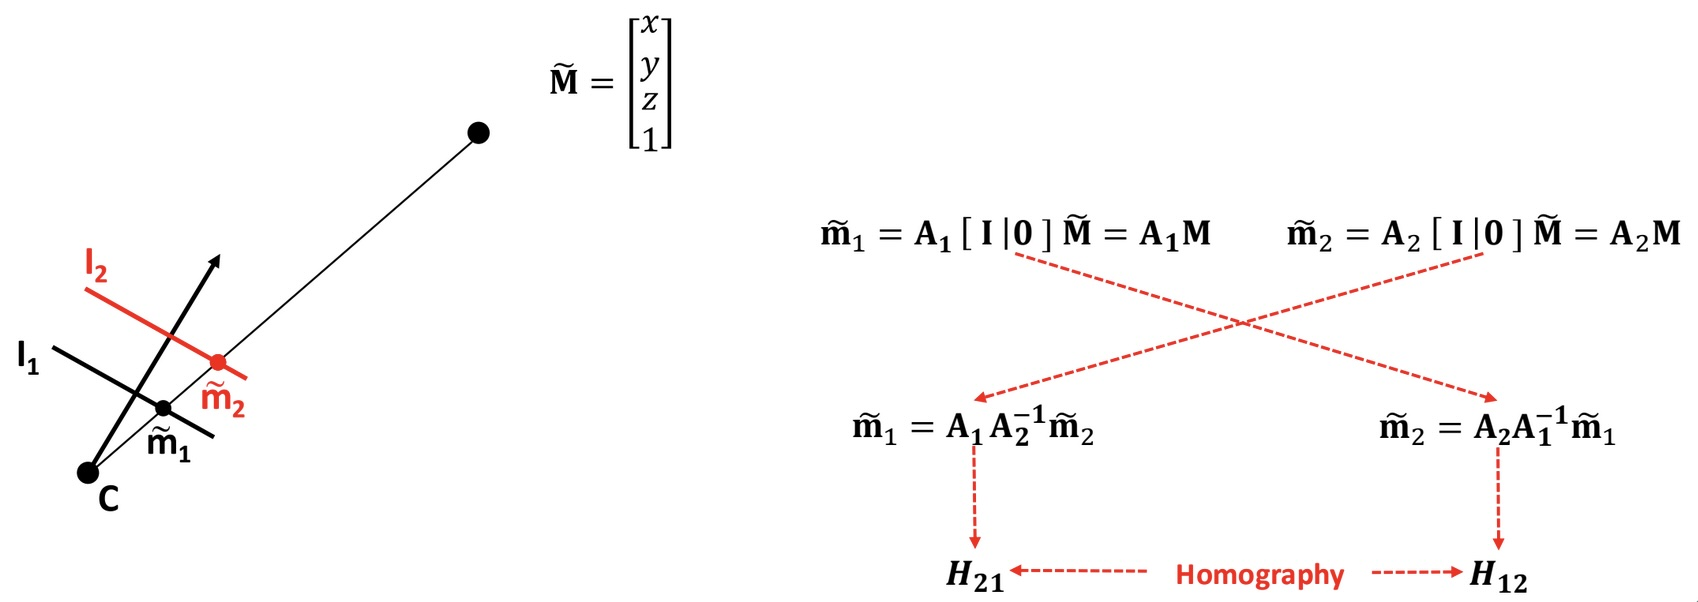
\includegraphics[width=0.8\linewidth]{./img/moving_homography.jpg}
  \caption{Any two images taken by different cameras in fexed pose are related bu a homography}
  \label{fig:moving_homography}
\end{figure}

\subsubsection{Lens distortion}

The Perspective Projection Matrix is based on the pinhole camera model, however, real lenses introduce distortions with respect to the pure pinhole model.
We also have lens distortion, which is modelled through additional parameters that don't alter the form of the Perspective Projection Matrix.

We have two types of lens distortion: barrel distortion which bends straight lines outwards, and pincushion distortion, which causes straight lines to curve inward.

\subsubsection{Calibration}

We now have the Perspective Projection Matrix camera model, which can be decomposed in:
\begin{itemize}
  \item Intrinsic parameter matrix $A$.
  \item Rotation matrix $R$.
  \item Translation vector $T$.
\end{itemize}

\textbf{Camera calibration} is the process where \textbf{all parameters defining the camera model are estimated} for a specific camera device.
Depending on the application, \textbf{either the Perspective Projection Matrix (PMM) only, or also its independent components} ($A$,$R$,$T$) need to be estimated.

There are many camera calibration algorithms, but the basic process always relies on setting up a linear system of equations given a set of known 3D-2D correspondences.
To obtain the correspondences we use calibration targets, which have easily detectable features.

The approaches can be split into:
\begin{itemize}
  \item Those relying on a single image containing a known pattern.
  \item Those relying on several different images of one given planar pattern.
\end{itemize}

Since in every frame we change the relative position of the camera and the pattern, we will have a different set of extrinsic parameter for each image.
We will have just one set of intrinsic parameter since the camera is always the same across the different pictures.

\subsubsection{Zhang's method for Camera Calibration}

We use a chessboard pattern of which we know the number of internal corners and the size of the squares.
Internal corners can be easily detected by standard algorithms, like the Harris corner detector.
Typically the camera is fixed and you move the calibration target in front of the camera.
The $[R\,T]$ are estimated with respect to the reference system attached to the target, but it changes alongside with the pattern.
In each image the 3D world reference frame is taken at the top-left corner of the pattern.
Each image requires its own estimate of the extrinstic parameters, as they are different from one to the other.
Due to the choice of the world reference frame associated with calibration images, in each of them we consider only 3D points with $z=0$.
The Perspective Projection Matrix boils down to a simpler transformation defined by an homography $3\times 3$ matrix, like with $P$ as a homography.

$$k\tilde{m} = \tilde{P}\tilde{w}
\begin{bmatrix}
  p_{1,1} & p_{1,2} & \cancel{p_{1,3}} & p_{1,4} \\
  p_{2,1} & p_{2,2} & \cancel{p_{2,3}} & p_{2,4} \\
  p_{3,1} & p_{3,2} & \cancel{p_{3,3}} & p_{3,4} 
\end{bmatrix}
\begin{bmatrix}
x \\ y \\ \cancel{0} \\ 1
\end{bmatrix}
=
\begin{bmatrix}
  p_{1,1} & p_{1,2} & p_{1,4} \\
  p_{2,1} & p_{2,2} & p_{2,4} \\
  p_{3,1} & p_{3,2} & p_{3,4} 
\end{bmatrix}
\begin{bmatrix}
x \\ y \\ 1
\end{bmatrix}
= H\tilde{M}
$$

\paragraph{Estimating $H_i$ (DLT algorithm)}
Given a pattern with $m$ corners, we can write $m$ systems of 3 linear equations, where:
\begin{itemize}
  \item Both 3D as well as 2D coordinates are known due to the corners having been detected in the i-th image and the unknowns are thus the 9 elements in $H_i$.
  \item $H_i$ (and $P_i$ alike) is known up to an arbitrary scale factor, the independent elements in $H_i$ are 8.
\end{itemize}

\textbf{There are plenty of methods for the estimation}

The Zhang's method can be summarized as:
\begin{enumerate}
  \item Acquire $n$ images of a planar pattern with $m$ internal corners.
  \item For each image compute an initial guess for homography $H_i$.
  \item Refine eaech $H_i$ by minimizing the reprojection error.
  \item Get an initial guess for $A$ given the homographies $H_i$.
  \item Given $A$ and $H_i$, get an initial guess for $R_i$ and $T_i$.
  \item Compute an initial guess for lens distortion parameters $k$.
  \item Refine all parameters $A$, $R_i$, $T_i$, $k$ by minimizing the reprojection error.
\end{enumerate}

\subsubsection{Image warping}

After applying the warping function you get real coordinates not discrete ones.
During the mapping, some pixels of the destination image may be not rounded perfectly.
What if more pixels go to the same position?
\begin{figure}[htbp]
  \centering
  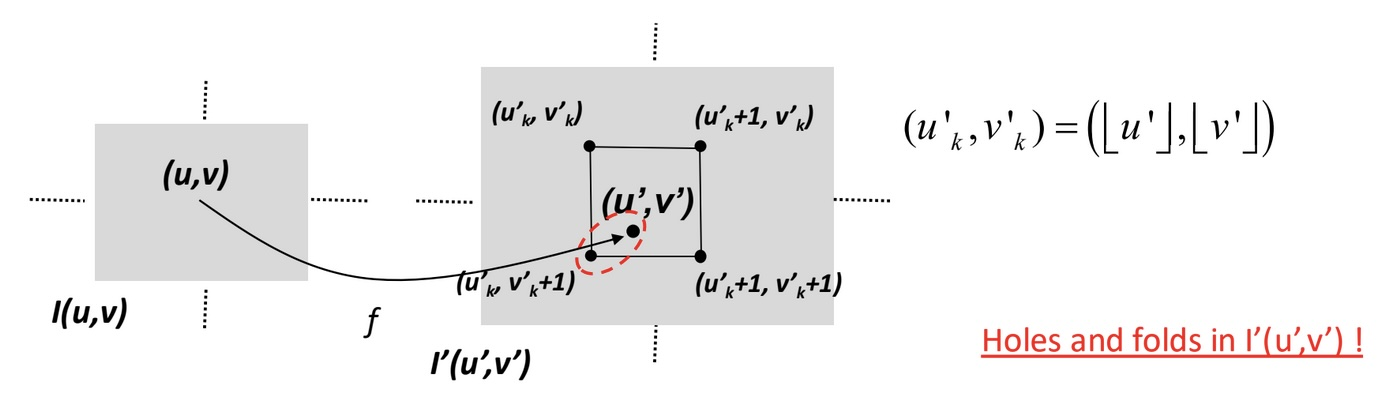
\includegraphics[width=0.8\linewidth]{./img/forward_mapping.jpg}
  \caption{A better choice consists in mapping to the closest point into the destination image}
  \label{fig:forward_mapping}
\end{figure}

Since the coordinates are always real values the different mapping strategies can be to map the closest point or to interpolate between the 4 closest points.
